\documentclass{article}
\usepackage[utf8]{inputenc}
\usepackage{amsmath}
\usepackage{graphicx}
\usepackage{hyperref}
\usepackage[english]{babel}\usepackage{subcaption}
\usepackage{sidecap}
\usepackage{lipsum}
\usepackage{multicol}
\usepackage{sectsty}
\usepackage{caption}
\usepackage{placeins}
\usepackage{subcaption}
\usepackage{bm}
\usepackage[dvipsnames]{xcolor}

\definecolor{myred}{RGB}{143, 42, 12}
\definecolor{myblue}{RGB}{58, 83, 197}
\definecolor{myorange}{RGB}{219, 146, 0}
\newcommand{\centered}[1]{\begin{tabular}{l} #1 \end{tabular}}



% \sectionfont{\centering}
\usepackage[a4paper,top=2cm,bottom=2cm,left=2cm,right=2cm]{geometry}
\title{\textbf{Robotics II} \\ \large{\textbf{Final Project}}}
\author{Marco Pennese 1749223, Veronica Vulcano 1760405}
\date{}

\begin{document}
\maketitle
\tableofcontents
\pagebreak

\section{Introduction}
aa
\section{1-dof arm under gravity}
\paragraph{}We start our work by focusing on a simple robot arm (pendulum) under gravity.
\subsection{Simulation and dynamic model}
\paragraph{} We have implemented a scene from scratch in V-REP by taking a base, then a revolute joint and a link. We control the joint in position with the built-in PID controller using the default parameters. The arm is in the 0 position at rest. The link is a parallelepiped long 1 $m$ and has a transversal section that is a square with side equal to 0.1 $m$. The mass of the link is 5 $kg$ and the principal moment of inertia is $5\cdot1.667\cdot10^{-3}$ $kg\cdot m^2$. Since the arm has a uniform density, the center of mass is located at the center of the link, so it is 0.5 $m$ from the top. The physics engine used is ODE, because when we will use the API function simxGetJointForce, this will return the total force/torque applied to the joint along its $z$ axis.
\begin{figure}[!htbp]
\centering
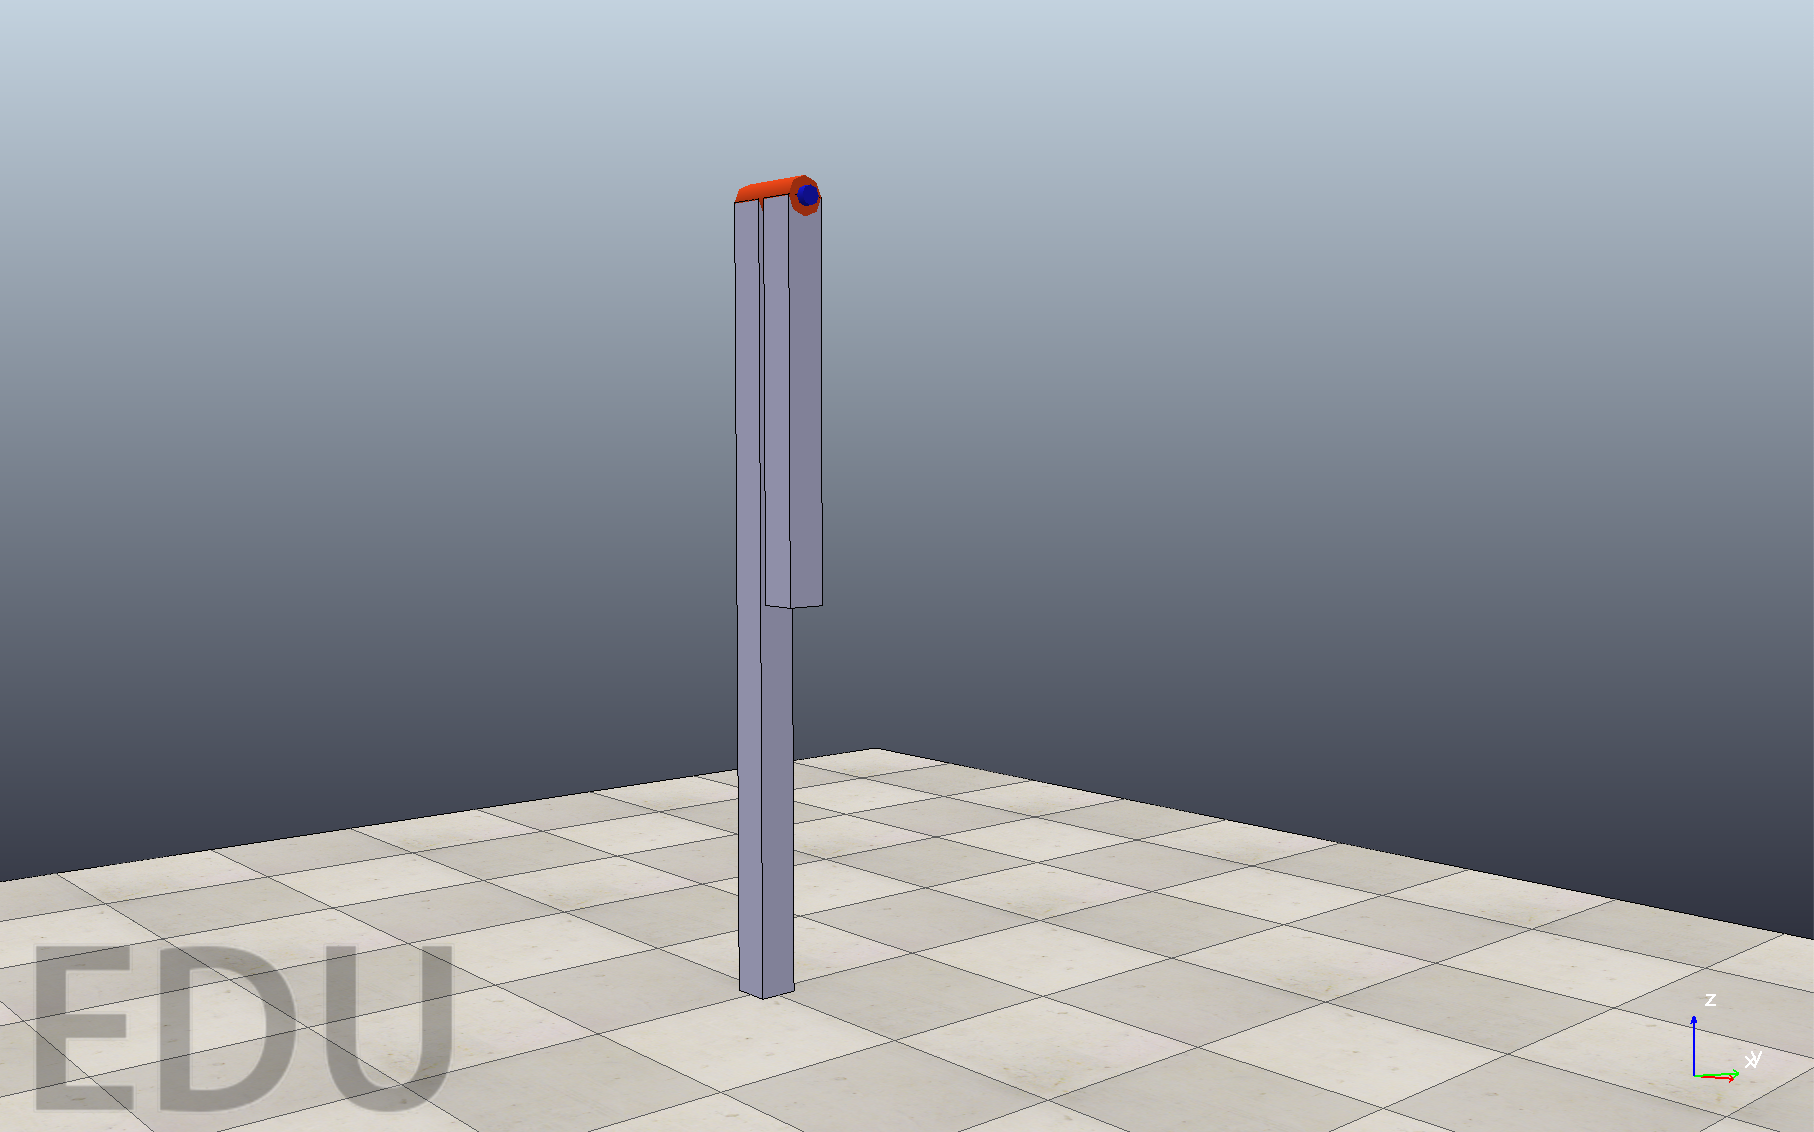
\includegraphics[width=0.7\textwidth]{images/1-dof/scene.png}
\caption{V-REP scene of the 1-dof robot arm}
\end{figure}
\FloatBarrier
The dynamic model is:

\[u=gmd \sin(q) + (I+md^2)\ddot{q}= \begin{bmatrix}
\sin(q) & \ddot{q}
\end{bmatrix}\begin{bmatrix}
gmd \\ I +md^2
\end{bmatrix}\]

Regarding the simulation, we have written a Matlab script in which we first connect to V-REP and then load the scene. In order to generate a trajectory made by the combination of sines and cosines, there is a function called generate\_exciting\_traj() that generates a random exciting trajectory.

\[q_j(t) = \sum_{l=1}^{L}{\frac{ a_{l,j}}{ l\omega_f }\sin(l\omega_f t)-\frac{ b_{l,j}}{l\omega_f}\cos(l\omega_f t)+q_{0,j}}\]

\noindent with $L = 5$ and $\omega_f = 0.1\pi$. However, we have started with simpler trajectories generated through the function looping\_splines(),which makes an interpolation of some given positions and instants of time with a cubic splines.
\\\\
After generated a trajectory, the simulation starts. In the main loop we first get the joint position, velocity and torque (with –); then, we set a new target position according to the trajectory and the instant of time.
\\\\
We obtain the measured accelerations through differentiation; this led to somewhat noisy values. In order to compensate for this, we apply a low-pass filter of order 16 and cutoff frequency equal to $0.35*\pi$. Also the measured torques are noisy, so we apply the same filter.
\paragraph{}After that, we have all the ingredients to generate the regressor matrix with all the computed values by staking all the $Y$ in a unique matrix. We do the same for the measured torques.

\subsection{Experiments}
\paragraph{Experiment 1}We have started from a very simple trajectory according to which the robot has to move from the 0 position to $\frac{\pi}{4}$ and then go back to the 0 position in 20 seconds. The function used to generate this trajectory is looping\_splines().

\begin{figure}[!htbp]
\centering
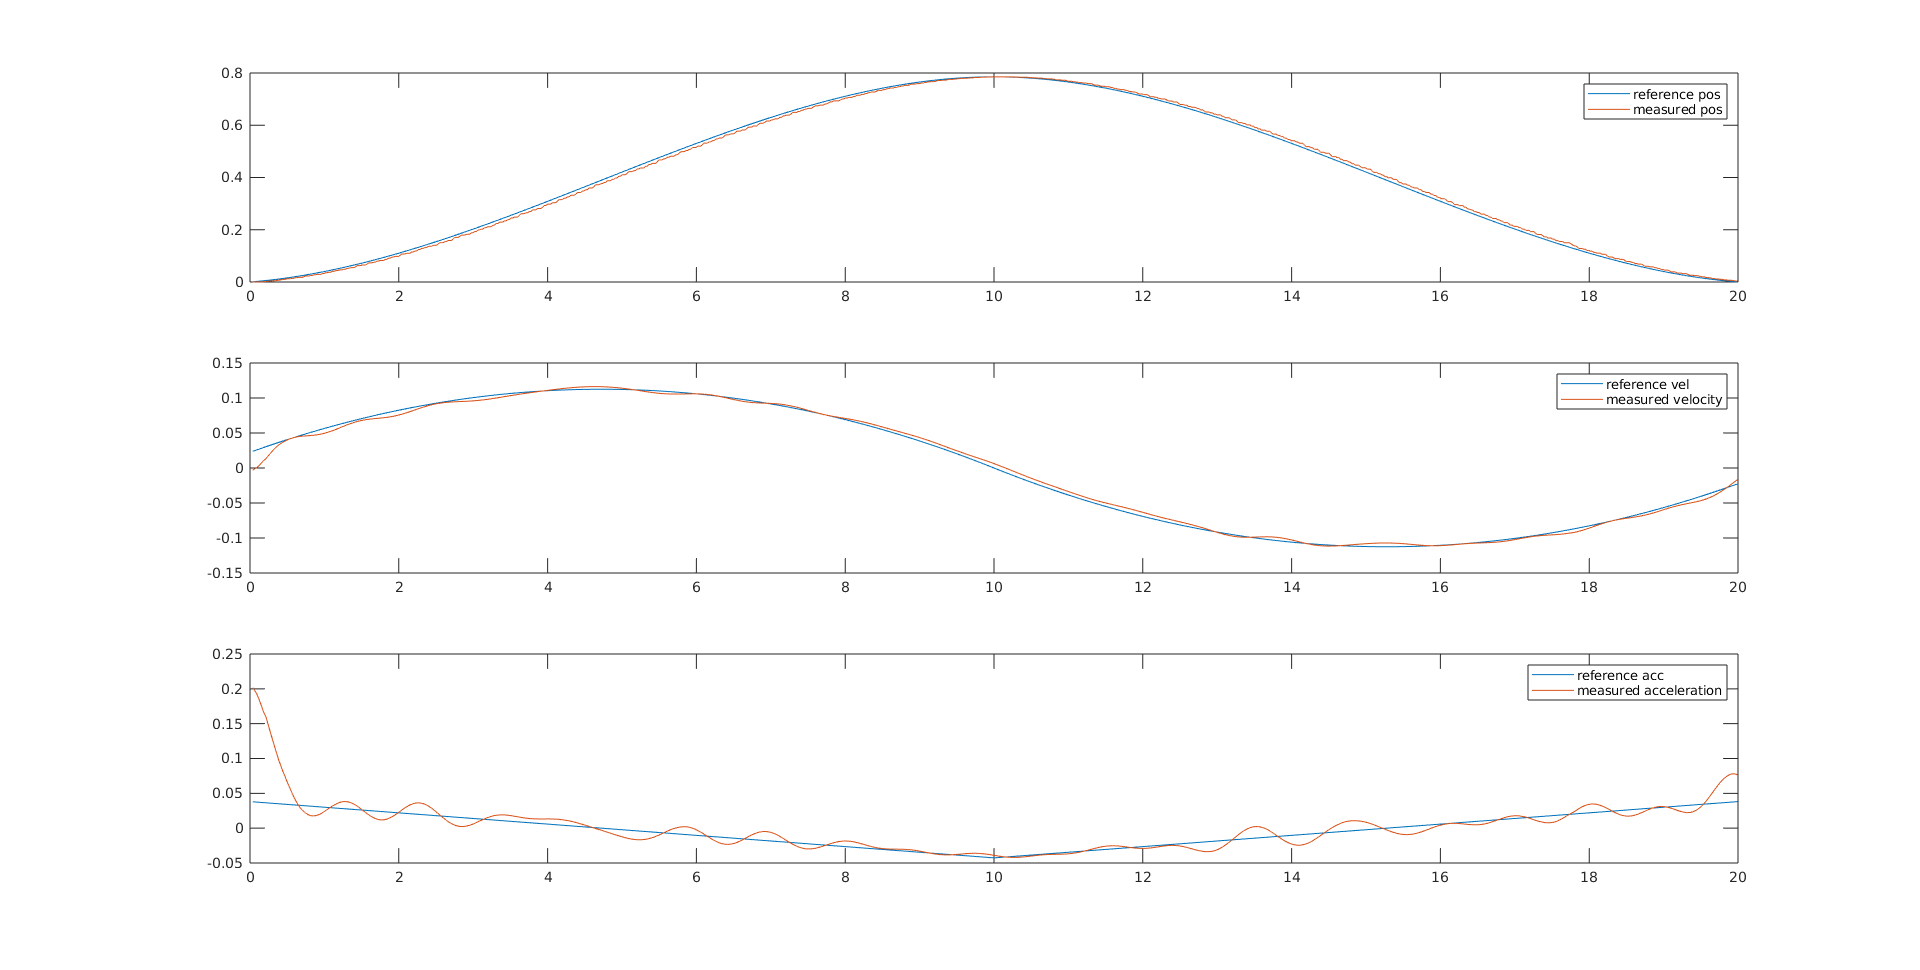
\includegraphics[width=0.7\textwidth]{images/1-dof/new_experiment1_traj.png}
\caption{Plot of the reference position, velocity and acceleration vs measured position, velocity and acceleration (filtered)}
\end{figure}

\noindent With this trajectory we obtain a torque which is always positive:

\begin{figure}[!htbp]
\centering
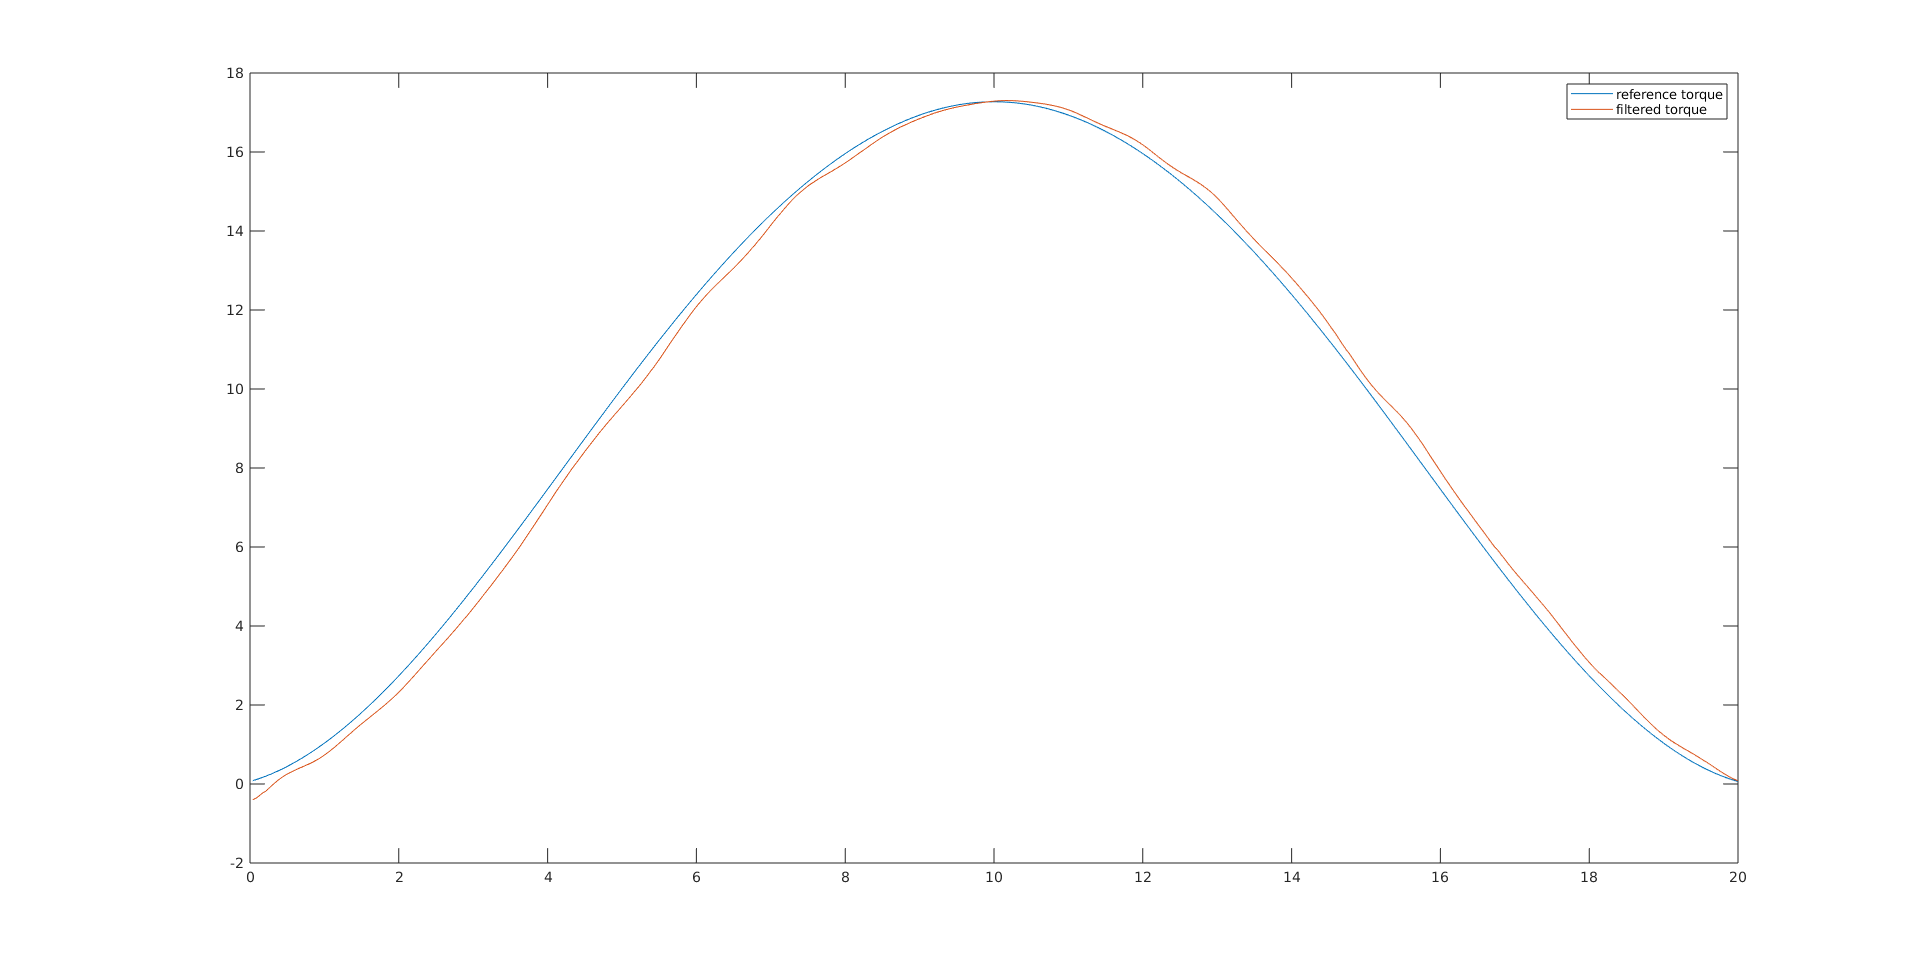
\includegraphics[width=0.7\textwidth]{images/1-dof/new_experiment1.png}
\caption{Plot of the reference torque vs measured torque (filtered)}
\end{figure}
\pagebreak
\paragraph{Experiment 2}Then, we move to a more complex trajectory according to which the robot has to move from the 0 position to $\frac{\pi}{4}$, then go to $-\frac{\pi}{4}$ and finally return in the 0 position in 20 seconds. The function used to generate this trajectory is looping\_splines() as before.

\begin{figure}[!htbp]
\centering
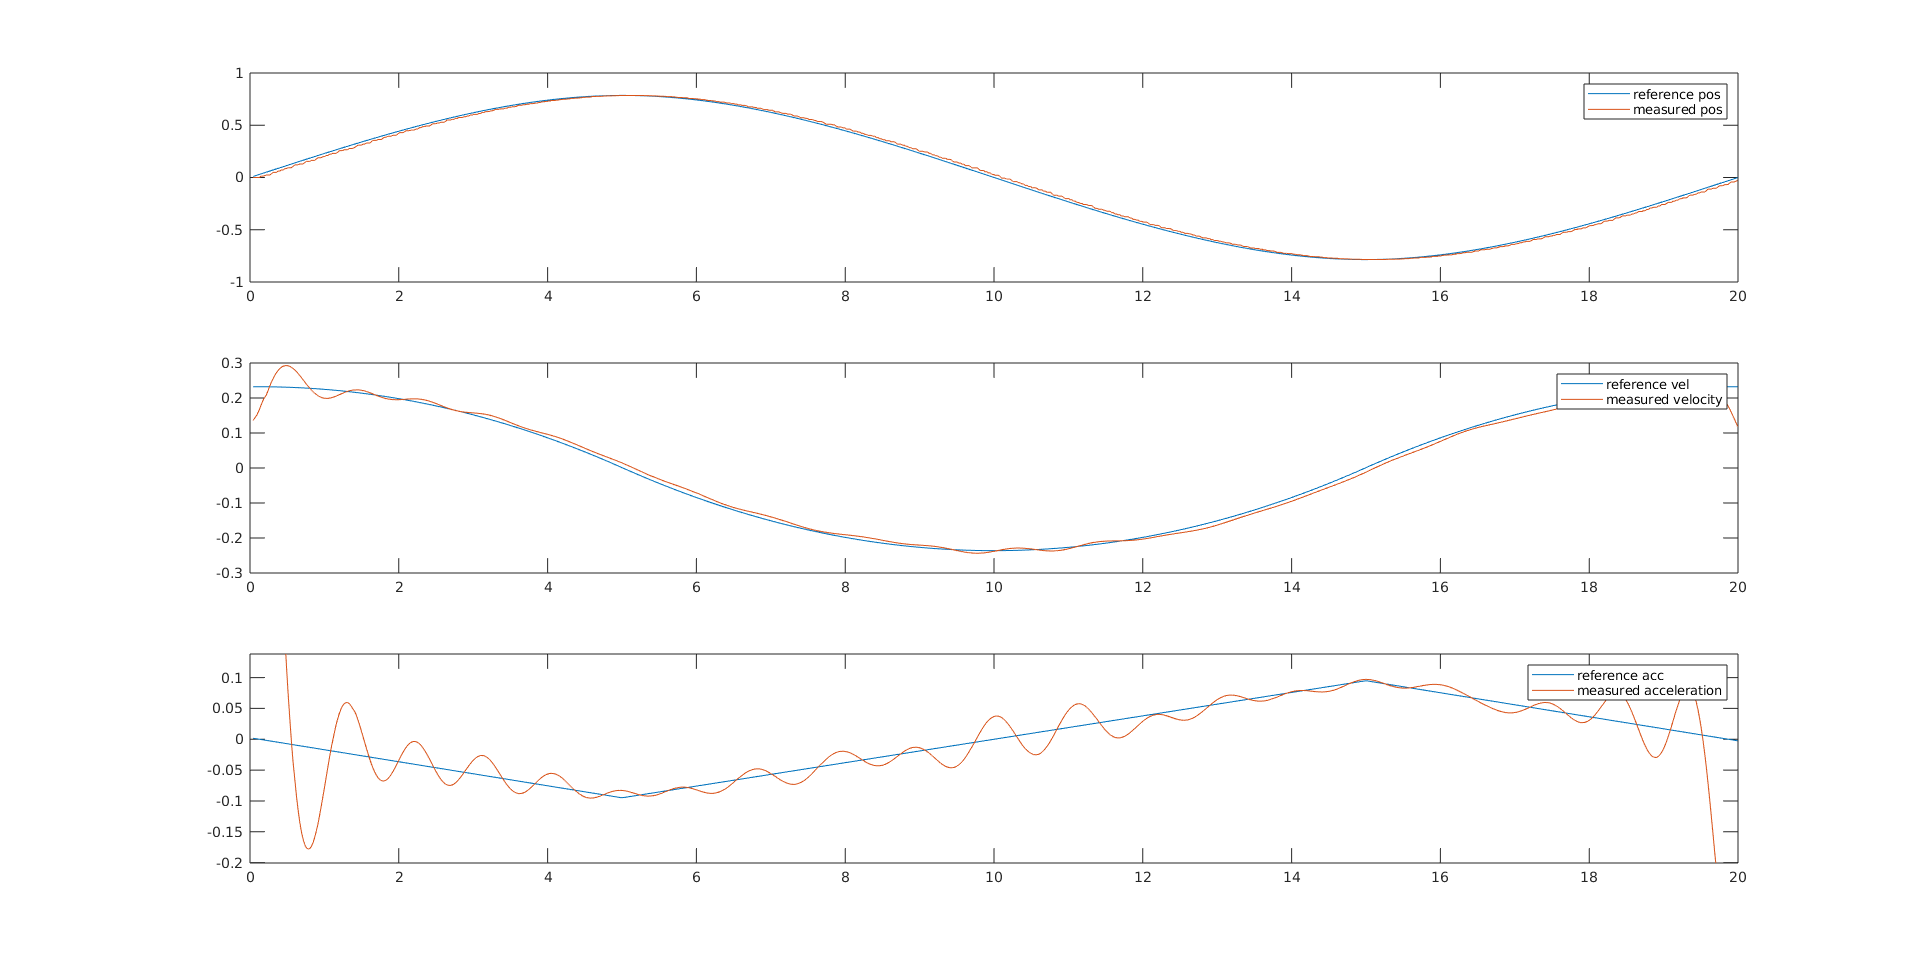
\includegraphics[width=0.7\textwidth]{images/1-dof/new_experiment2_traj.png}
\caption{Plot of the reference position, velocity and acceleration vs measured position, velocity and acceleration (filtered)}
\end{figure}
\FloatBarrier

\noindent With this trajectory we obtain a torque which is positive in the first half wave and negative in the second half wave:

\begin{figure}[!htbp]
\centering
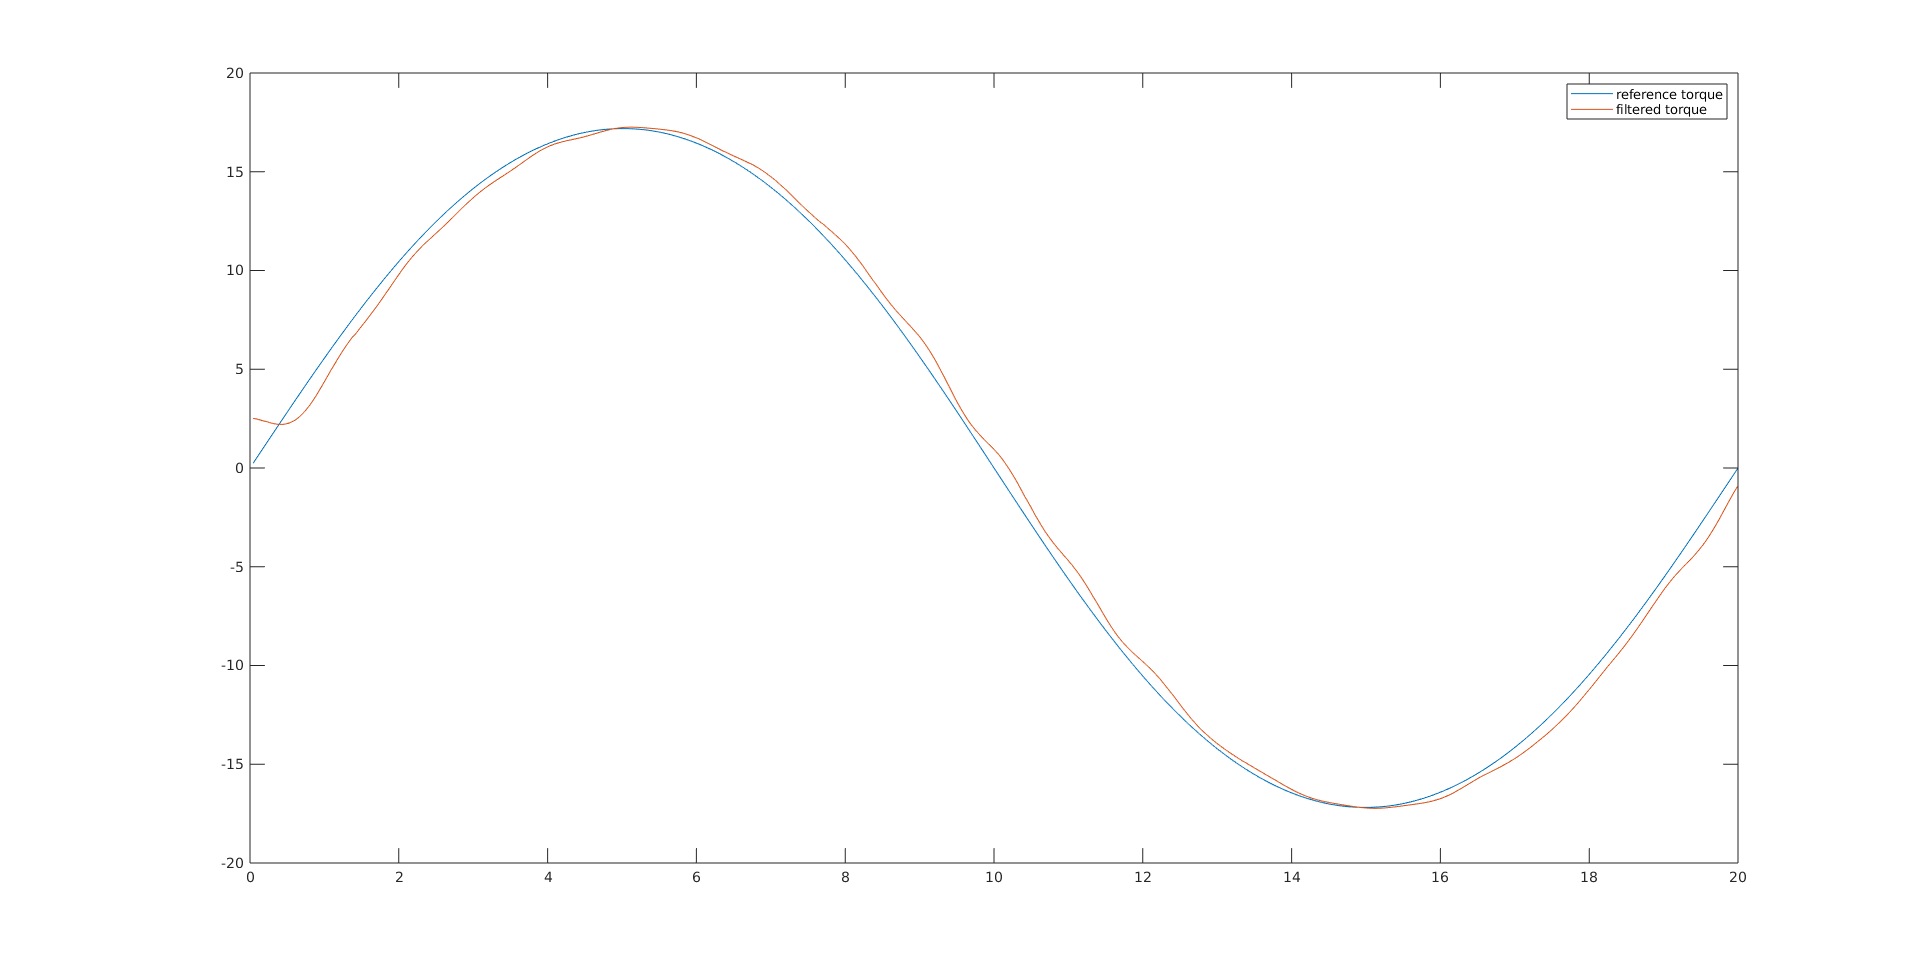
\includegraphics[width=0.7\textwidth]{images/1-dof/new_experiment2.png}
\caption{Plot of the reference torque vs measured torque (filtered)}
\end{figure}
\pagebreak

\paragraph{Experiment 3 and 4}Finally, we have generated two trajectories made by the combination of sines and cosines through the generate\_exciting\_traj() function. Both these trajectories are repeated 3 consecutive times. The results are reported below.
\paragraph{}Trajectory one:

\begin{figure}[!htbp]
\centering
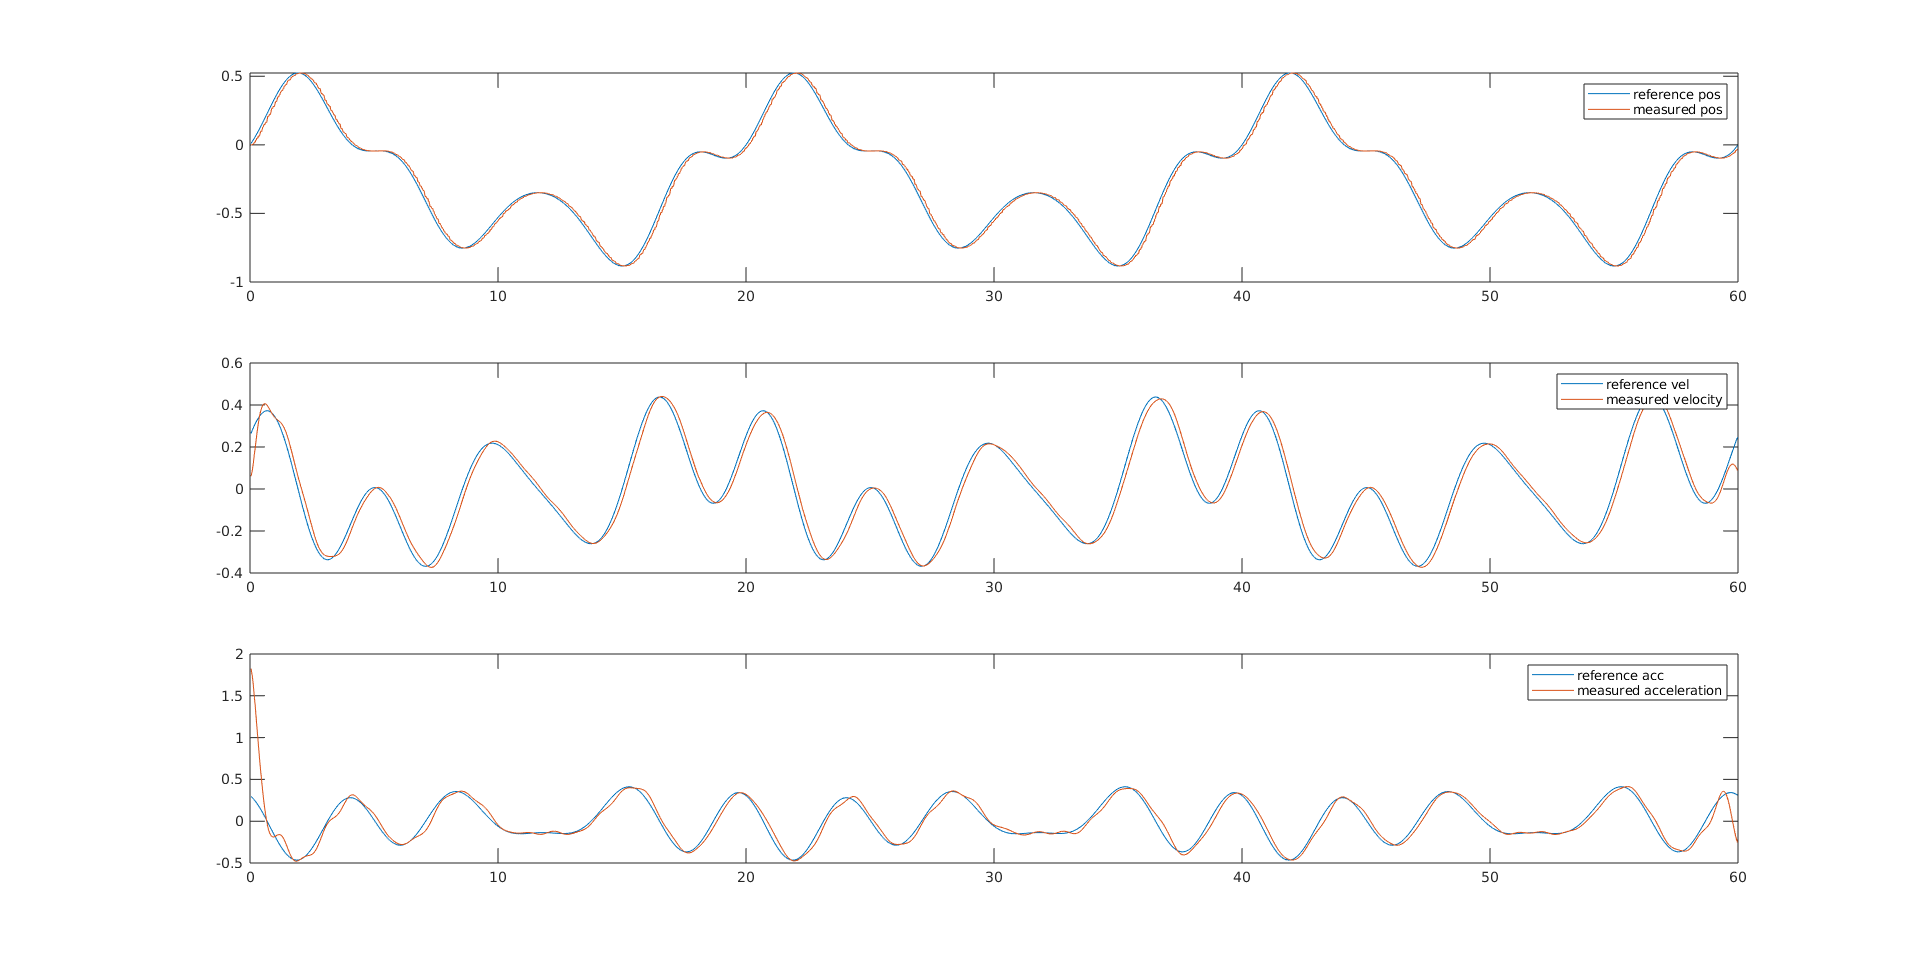
\includegraphics[width=0.7\textwidth]{images/1-dof/new_experiment3_traj.png}
\caption{Plot of the reference position, velocity and acceleration vs measured position, velocity and acceleration (filtered)}
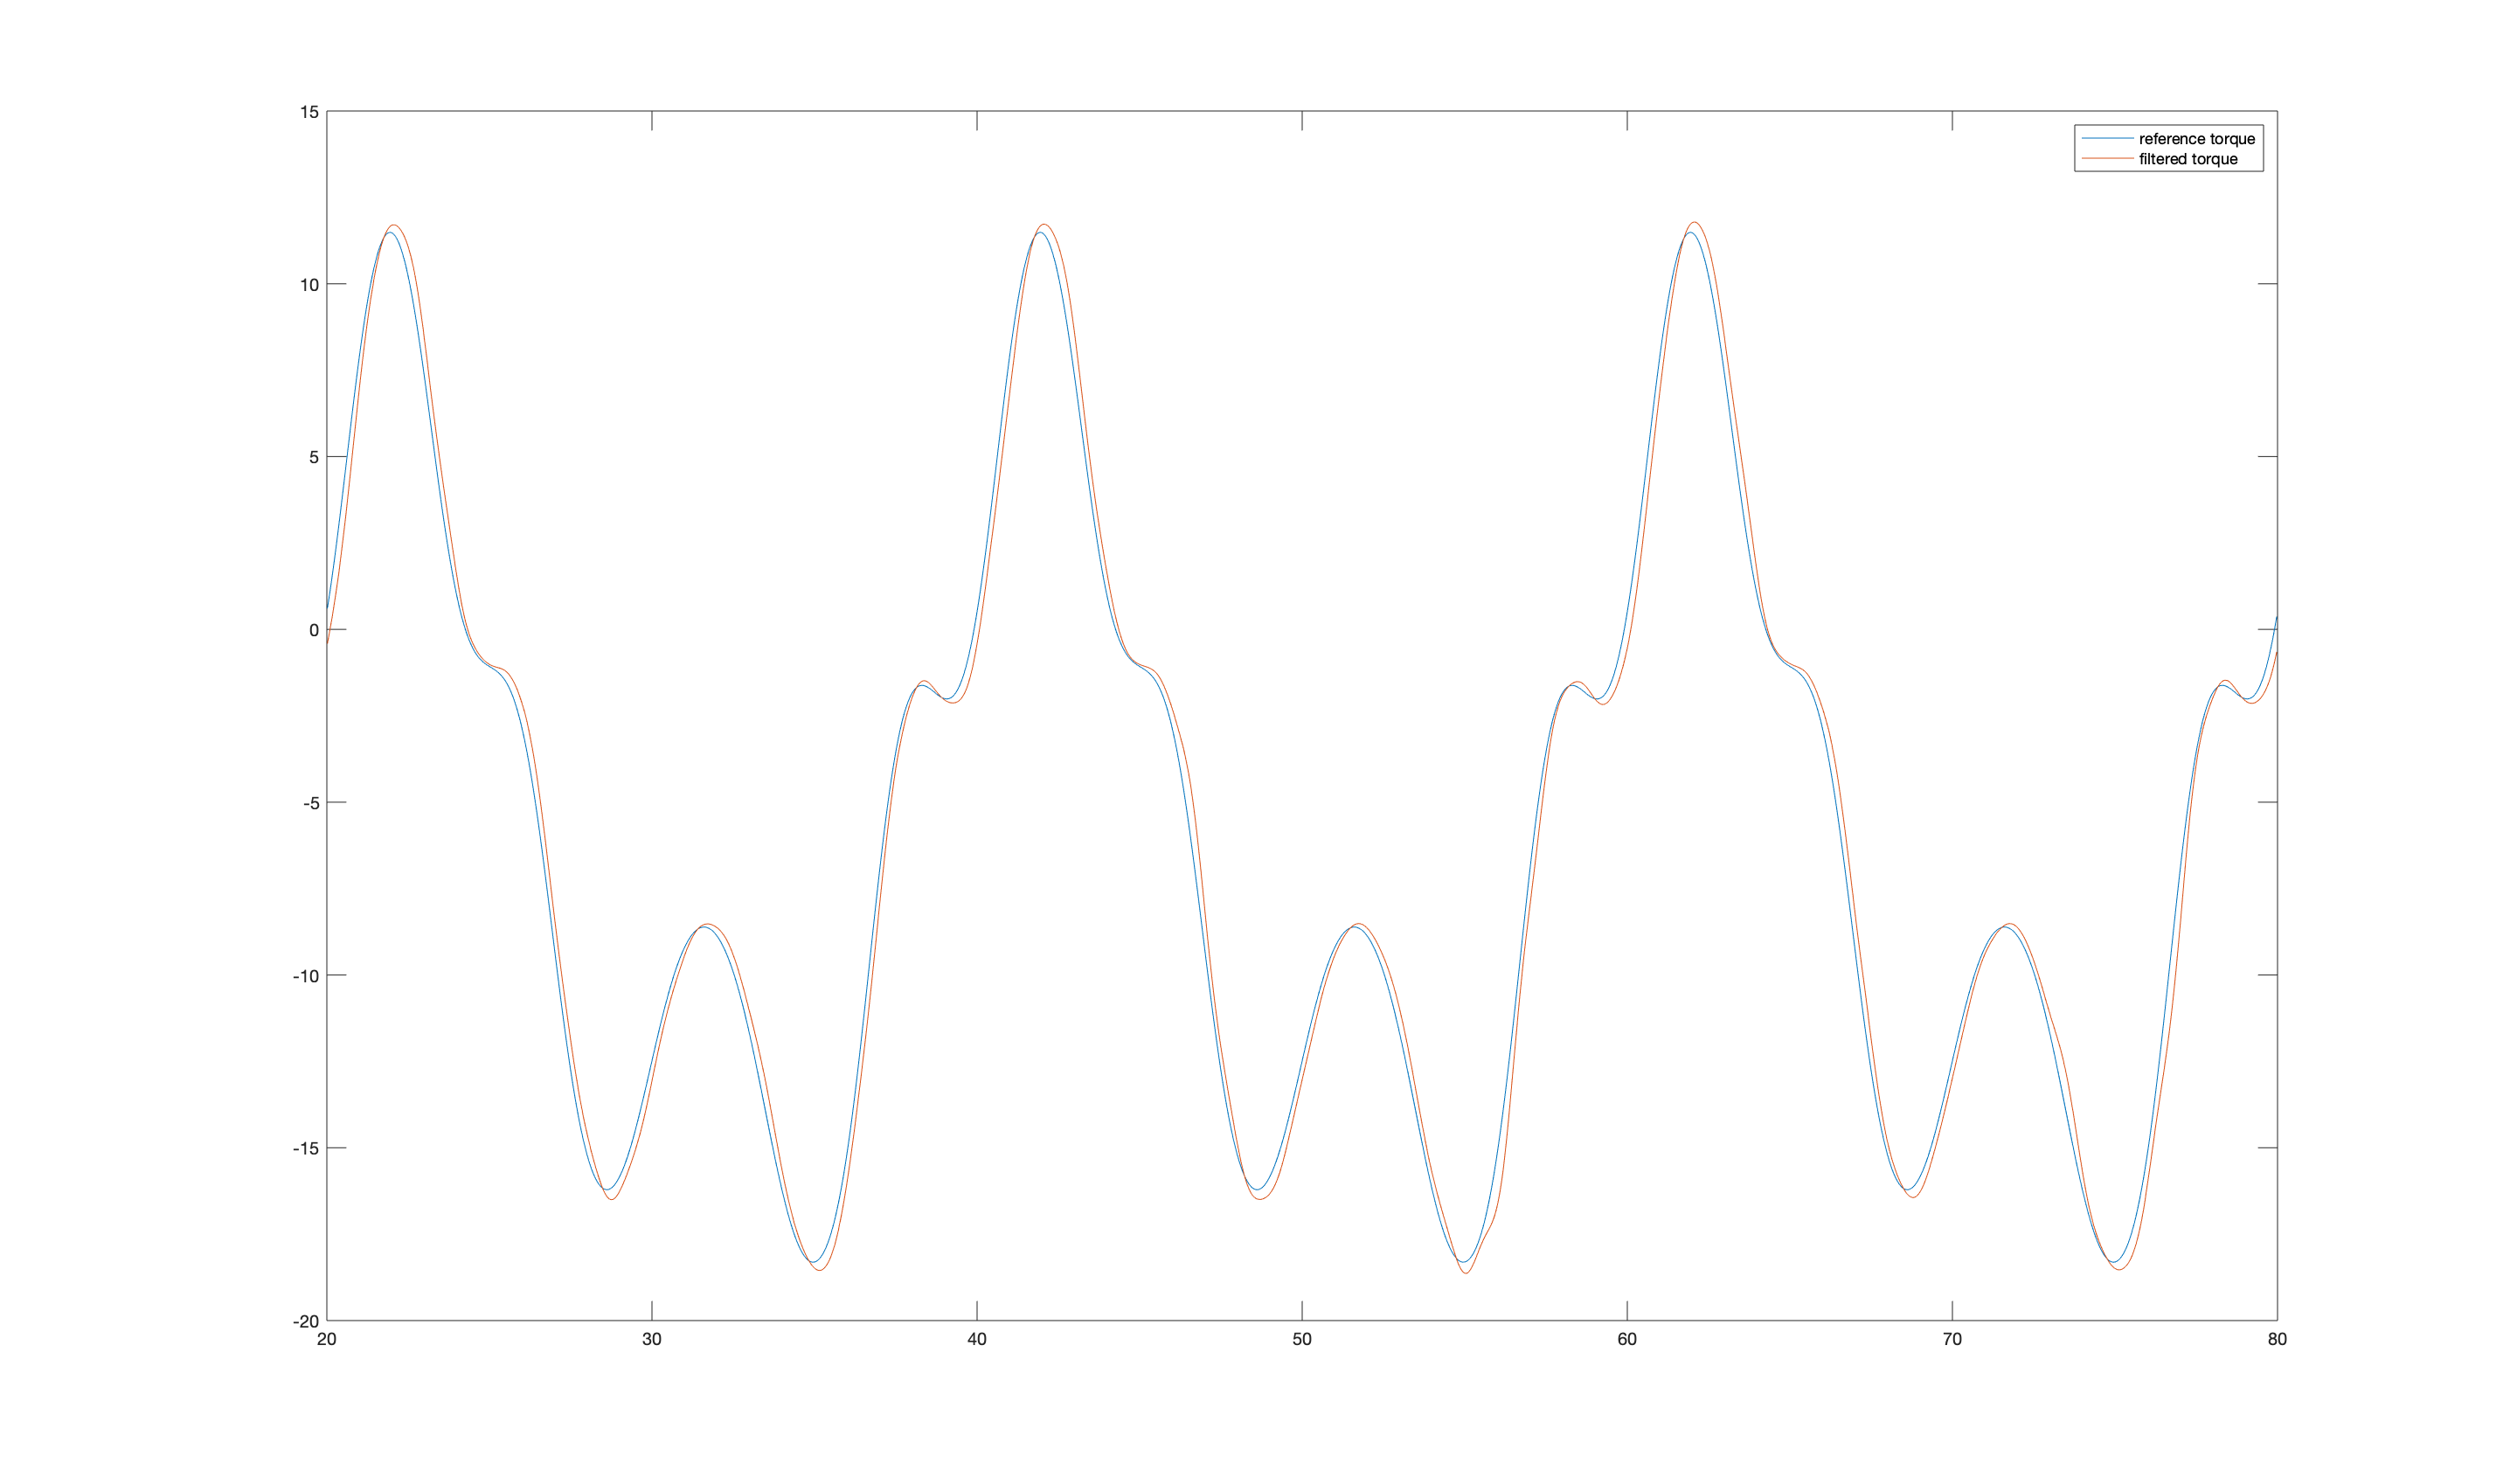
\includegraphics[width=0.7\textwidth]{images/1-dof/new_experiment3.png}
\caption{Plot of the reference torque vs measured torque (filtered)}
\end{figure}
\FloatBarrier

\pagebreak
\paragraph{}Trajectory two:

\begin{figure}[!htbp]
\centering
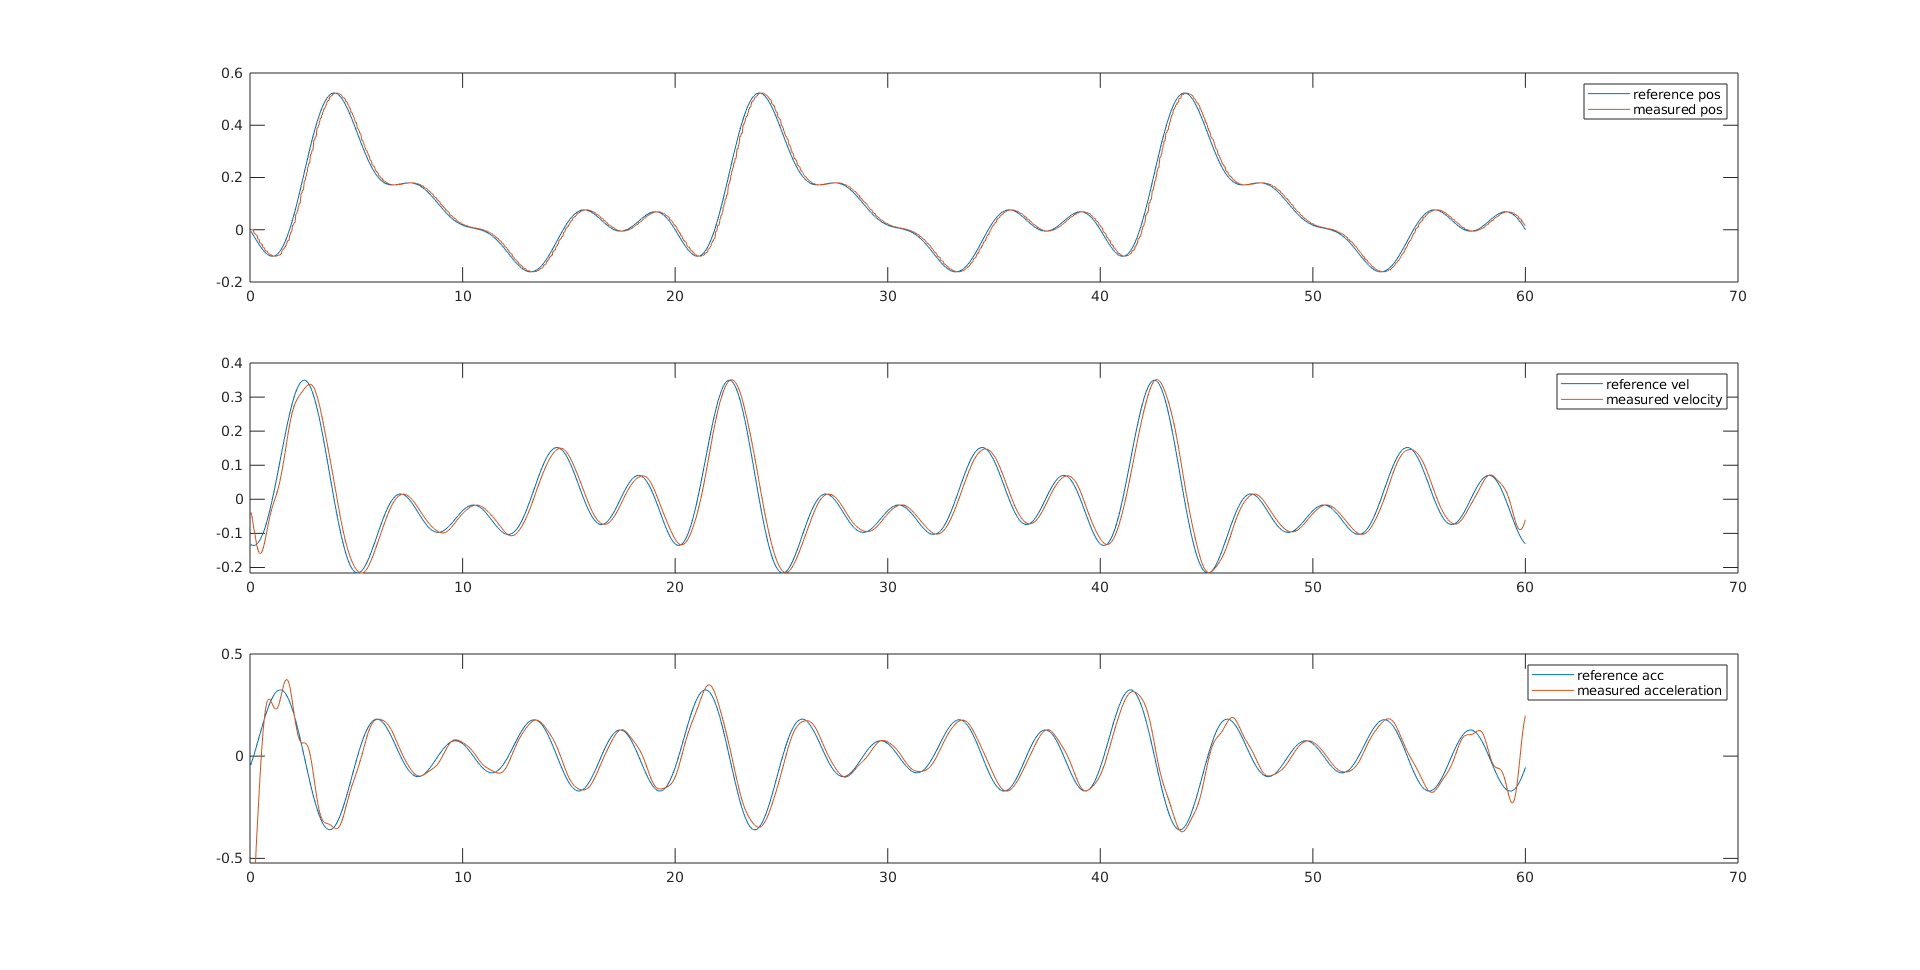
\includegraphics[width=0.7\textwidth]{images/1-dof/new_experiment4_traj.png}
\caption{Plot of the reference position, velocity and acceleration vs measured position, velocity and acceleration (filtered)}
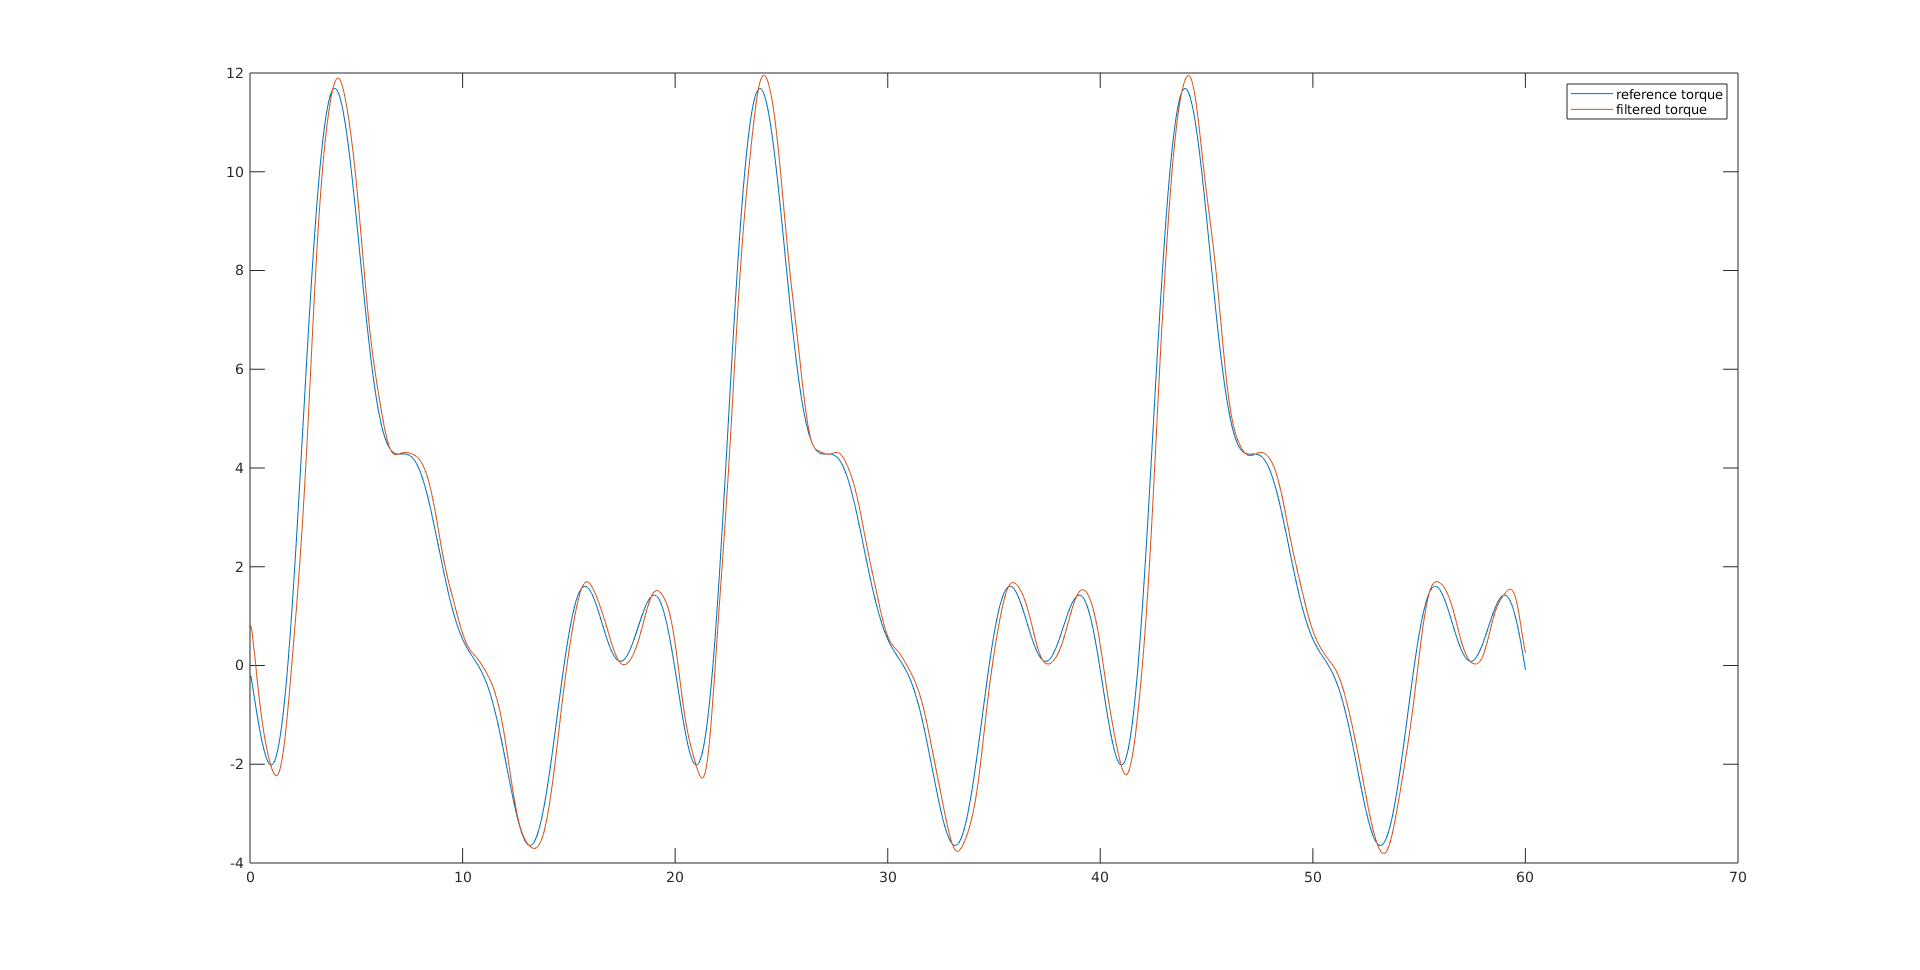
\includegraphics[width=0.7\textwidth]{images/1-dof/new_experiment4.png}
\caption{Plot of the reference torque vs measured torque (filtered)}
\end{figure}
\FloatBarrier

\subsection{PBRP algorithm}
\paragraph{}If we had torque signs, we would apply directly the Penalty-Based Parameters Retrivial (PBRP) algorithm. The aim of this algorithm is to get a physically consistent set of parameters; in order to do so, we need to solve the following optimization problem:
\[\min_{p_k}{\phi(p_k)} = \lVert \overline{Y}\pi(p_k)-\overline{\tau} \rVert^2\]

\noindent where $\overline{Y}$ is the stacked regressor, $\overline{\tau}$ is the stacked  torque measurements and $\pi(p_k)$ is the coefficients vector computed from the current parameters vector $p_k$.

\paragraph{}In order to obtain a physically consistent set of parameters, we should put constraints on the mass and on the inertia. Since we are dealing with a 1 dof robot, the only constraints we have is that both mass and inertia should be positive.

\[m > 0, I > 0\]

In general, it is possible to provide a set of lower and upper bounds for the dynamic parameters based on a priori knowledge. For instance, the center of mass must be inside the convex link of the robot. However, the aim of our work is to estimate the dynamic coefficients without torque signs. So, we cannot apply this algorithm directly, but we need a preliminary analysis in which we predict what is the most likely torque sign.

\subsection{Tree of solutions}
\paragraph{}First of all, we take the absolute values of the filtered measured torques. Then, we have to "mark" the function whenever it crosses 0. In order to do this, we should tolerate a threshold; we compute this threshold by discarding the 10\% of samples closer to 0. At this point, we discard all the samples under threshold; we are left with several segments so that in each of them the sign of the torque is either positive or negative.
\paragraph{}After that, we have to predict the torque sign for each segment. The idea is: we first take a random segment which could be either positive or negative, so we have two possible solutions; then, we take another segment which again could be either positive or negative, so at this stage we have four possible solutions (by considering the previous ones), and so on. This is an exponential problem, so if we have $n$ segments we would have $2^n$ possible solutions. However, it is possible to prevent the tree from being completely expanded because we can recognize in advance when a choice of sign lead to a wrong solution; in fact, when the PBRP algorithm is applied to a torque with the wrong sign, the loss should be higher than the one with the correct sign. So, at each level of the tree, we expand only the best nodes which are the ones with the lower loss until that segments (in our case, we decided to expand the best 5 nodes). For all the optimization problems of the tree we use pattern search algorithm because it is faster.
\paragraph{}At the end of this tree algorithm, we will obtain the best combination of signs for the segments sequence. So, we apply the PBRP algorithm to this sequence with a number of runs equal to 3 using simulated annealing.

\subsection{Results}
\paragraph{}In this section we are going to show the results obtained by applying the PBRP algorithm to the torques with the estimated signs.

\begin{table}[!htbp]
\centering
\begin{tabular}{|c|ccc|}
\hline
& $m$ & $d$ & $I$\\
\hline
Ground truth & 5 & 0.5 & 0.4208\\
Experiment 1 & 9.7053 & 0.2577 & 0.4116\\
Experiment 2 & 9.9157 & 0.2519 & 0\\
Experiment 3 & 6.9846 & 0.3577 & 0.0825\\
Experiment 4 & 6.3661 & 0.3915 & 0\\
\hline
\end{tabular}
\caption{Optimal solutions}
\end{table}

As we can see from the table, the optimal solutions that we get are quite different from the nominal values of the dynamic parameters. However, we are interested in the dynamic coefficients, so for each experiment, we will report the estimated dynamic coefficients compared with their ground values. In order to get a measure of the error, we decide to take the norm of the difference between these two vectors.

\paragraph{}We remember that:

\[\bm{\pi}= \begin{bmatrix}
\pi_1 \\ \pi_2
\end{bmatrix} = \begin{bmatrix}
gmd \\ I +md^2
\end{bmatrix}\]

The ground values of the dynamic coefficients are:

\[\begin{bmatrix}
\pi_1 \\ \pi_2
\end{bmatrix}=\begin{bmatrix}
24.5250 \\ 1.6708
\end{bmatrix}\]

\paragraph{Experiment 1} The estimated dynamic coefficients without torque signs are:

\[\begin{bmatrix}
\pi_1  \\ \pi_2 
\end{bmatrix}=\begin{bmatrix}
24.5312 \\ 1.0559
\end{bmatrix}\]

The norm of the error is 0.6149.

\begin{figure}[!htbp]
\centering
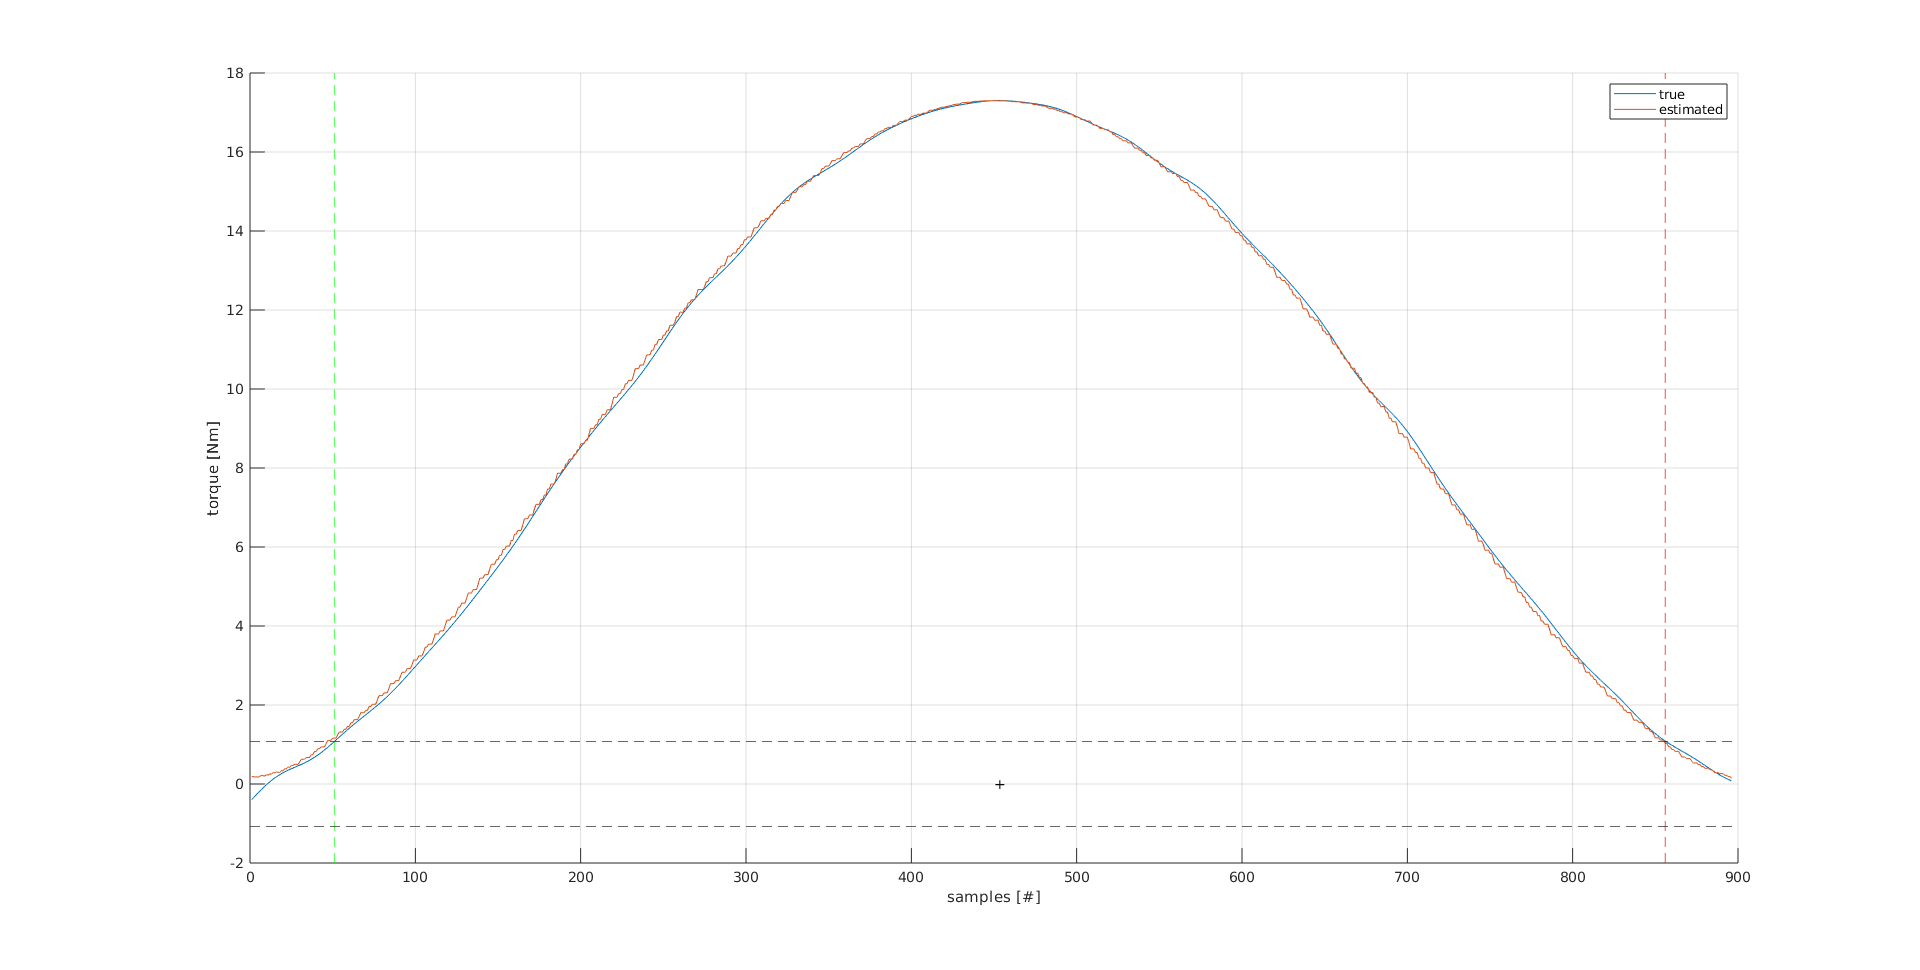
\includegraphics[width=0.8\textwidth]{images/1-dof/results_new_experiment1.png}
\caption{Plot of the reconstructed torque vs nominal torque. The gray dashed lines represent the threshold; the green dashed lines represent the start of the segment, while the red dashed lines represent the end of the segment. Samples under threshold are discarded. The signs estimated by the algorithm are reported for each segment.}
\end{figure}
\FloatBarrier
\paragraph{Experiment 2} The estimated dynamic coefficients without torque signs are:

\[\begin{bmatrix}
\pi_1  \\ \pi_2 
\end{bmatrix}=\begin{bmatrix}
24.4990 \\ 0.6290
\end{bmatrix}\]

The norm of the error is 1.0422.
\begin{figure}[!htbp]
\centering
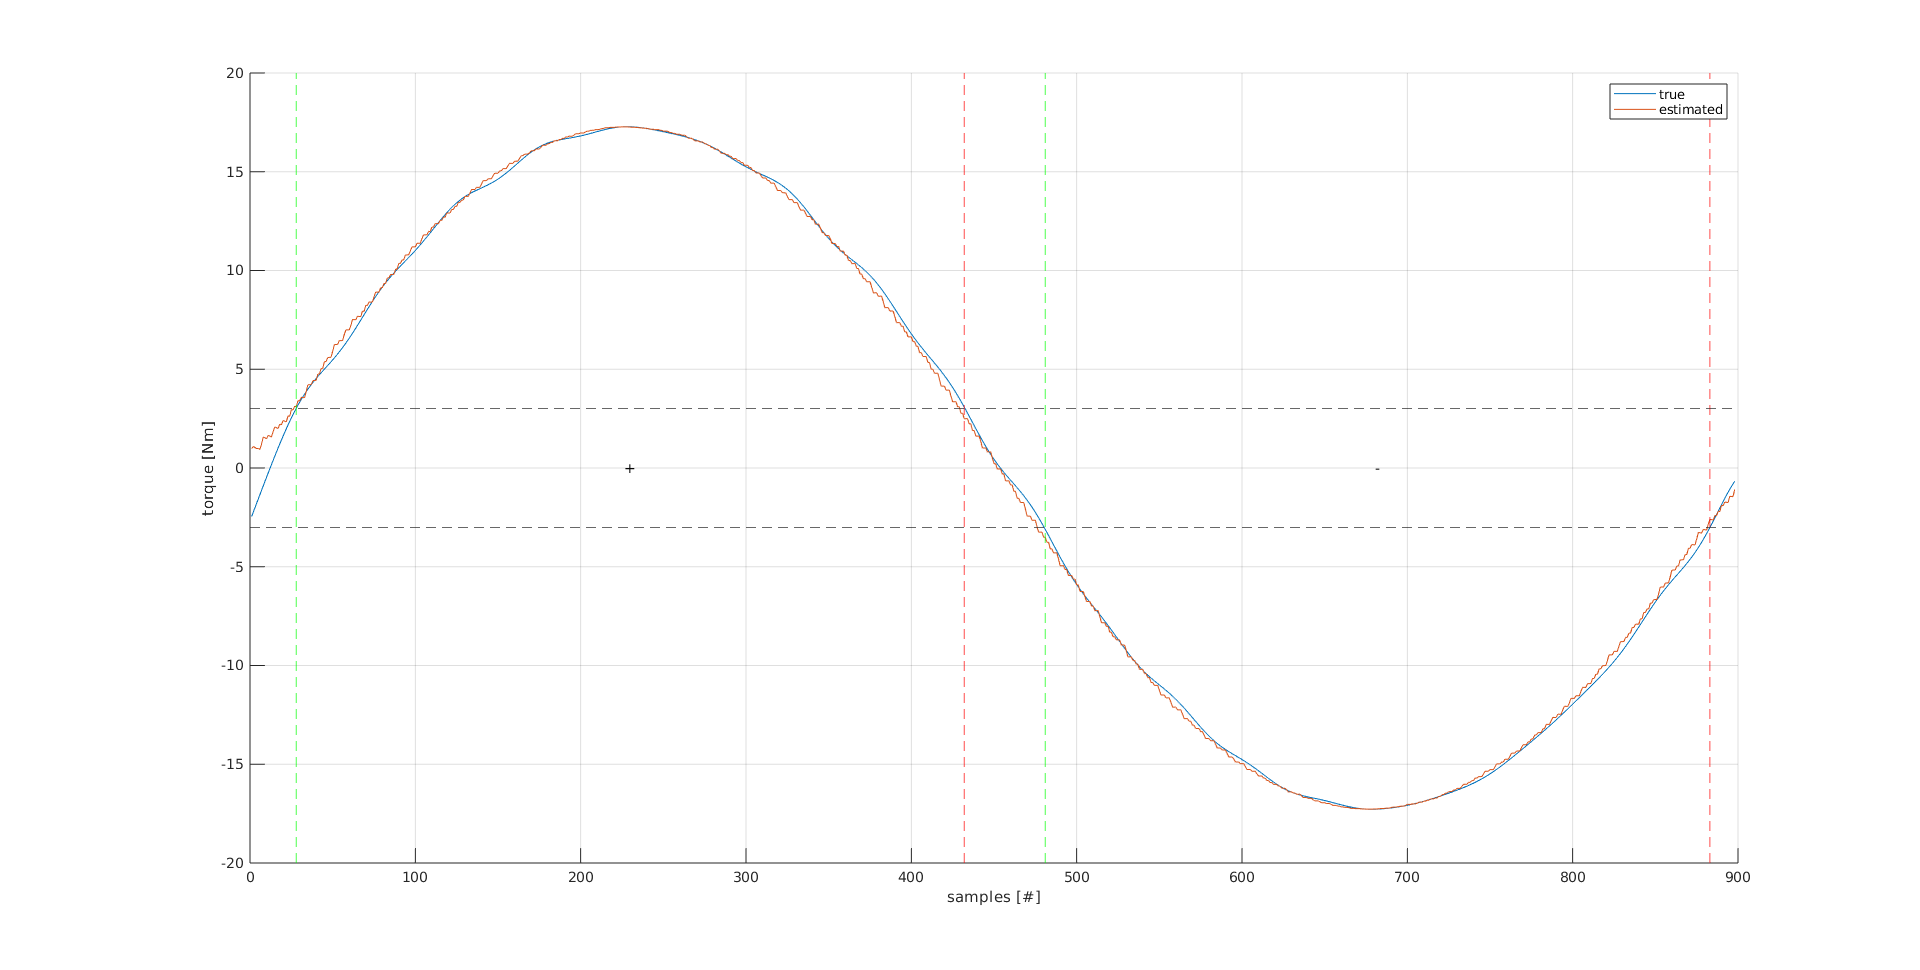
\includegraphics[width=0.8\textwidth]{images/1-dof/results_new_experiment2.png}
\caption{Plot of the reconstructed torque vs nominal torque. The gray dashed lines represent the threshold; the green dashed lines represent the start of the segment, while the red dashed lines represent the end of the segment. Samples under threshold are discarded. The signs estimated by the algorithm are reported for each segment.}
\end{figure}
\FloatBarrier
\paragraph{Experiment 3} The estimated dynamic coefficients without torque signs are:

\[\begin{bmatrix}
\pi_1  \\ \pi_2 
\end{bmatrix}=\begin{bmatrix}
24.5069 \\ 0.9760
\end{bmatrix}\]

The norm of the error is 0.6950.
\begin{figure}[!htbp]
\centering
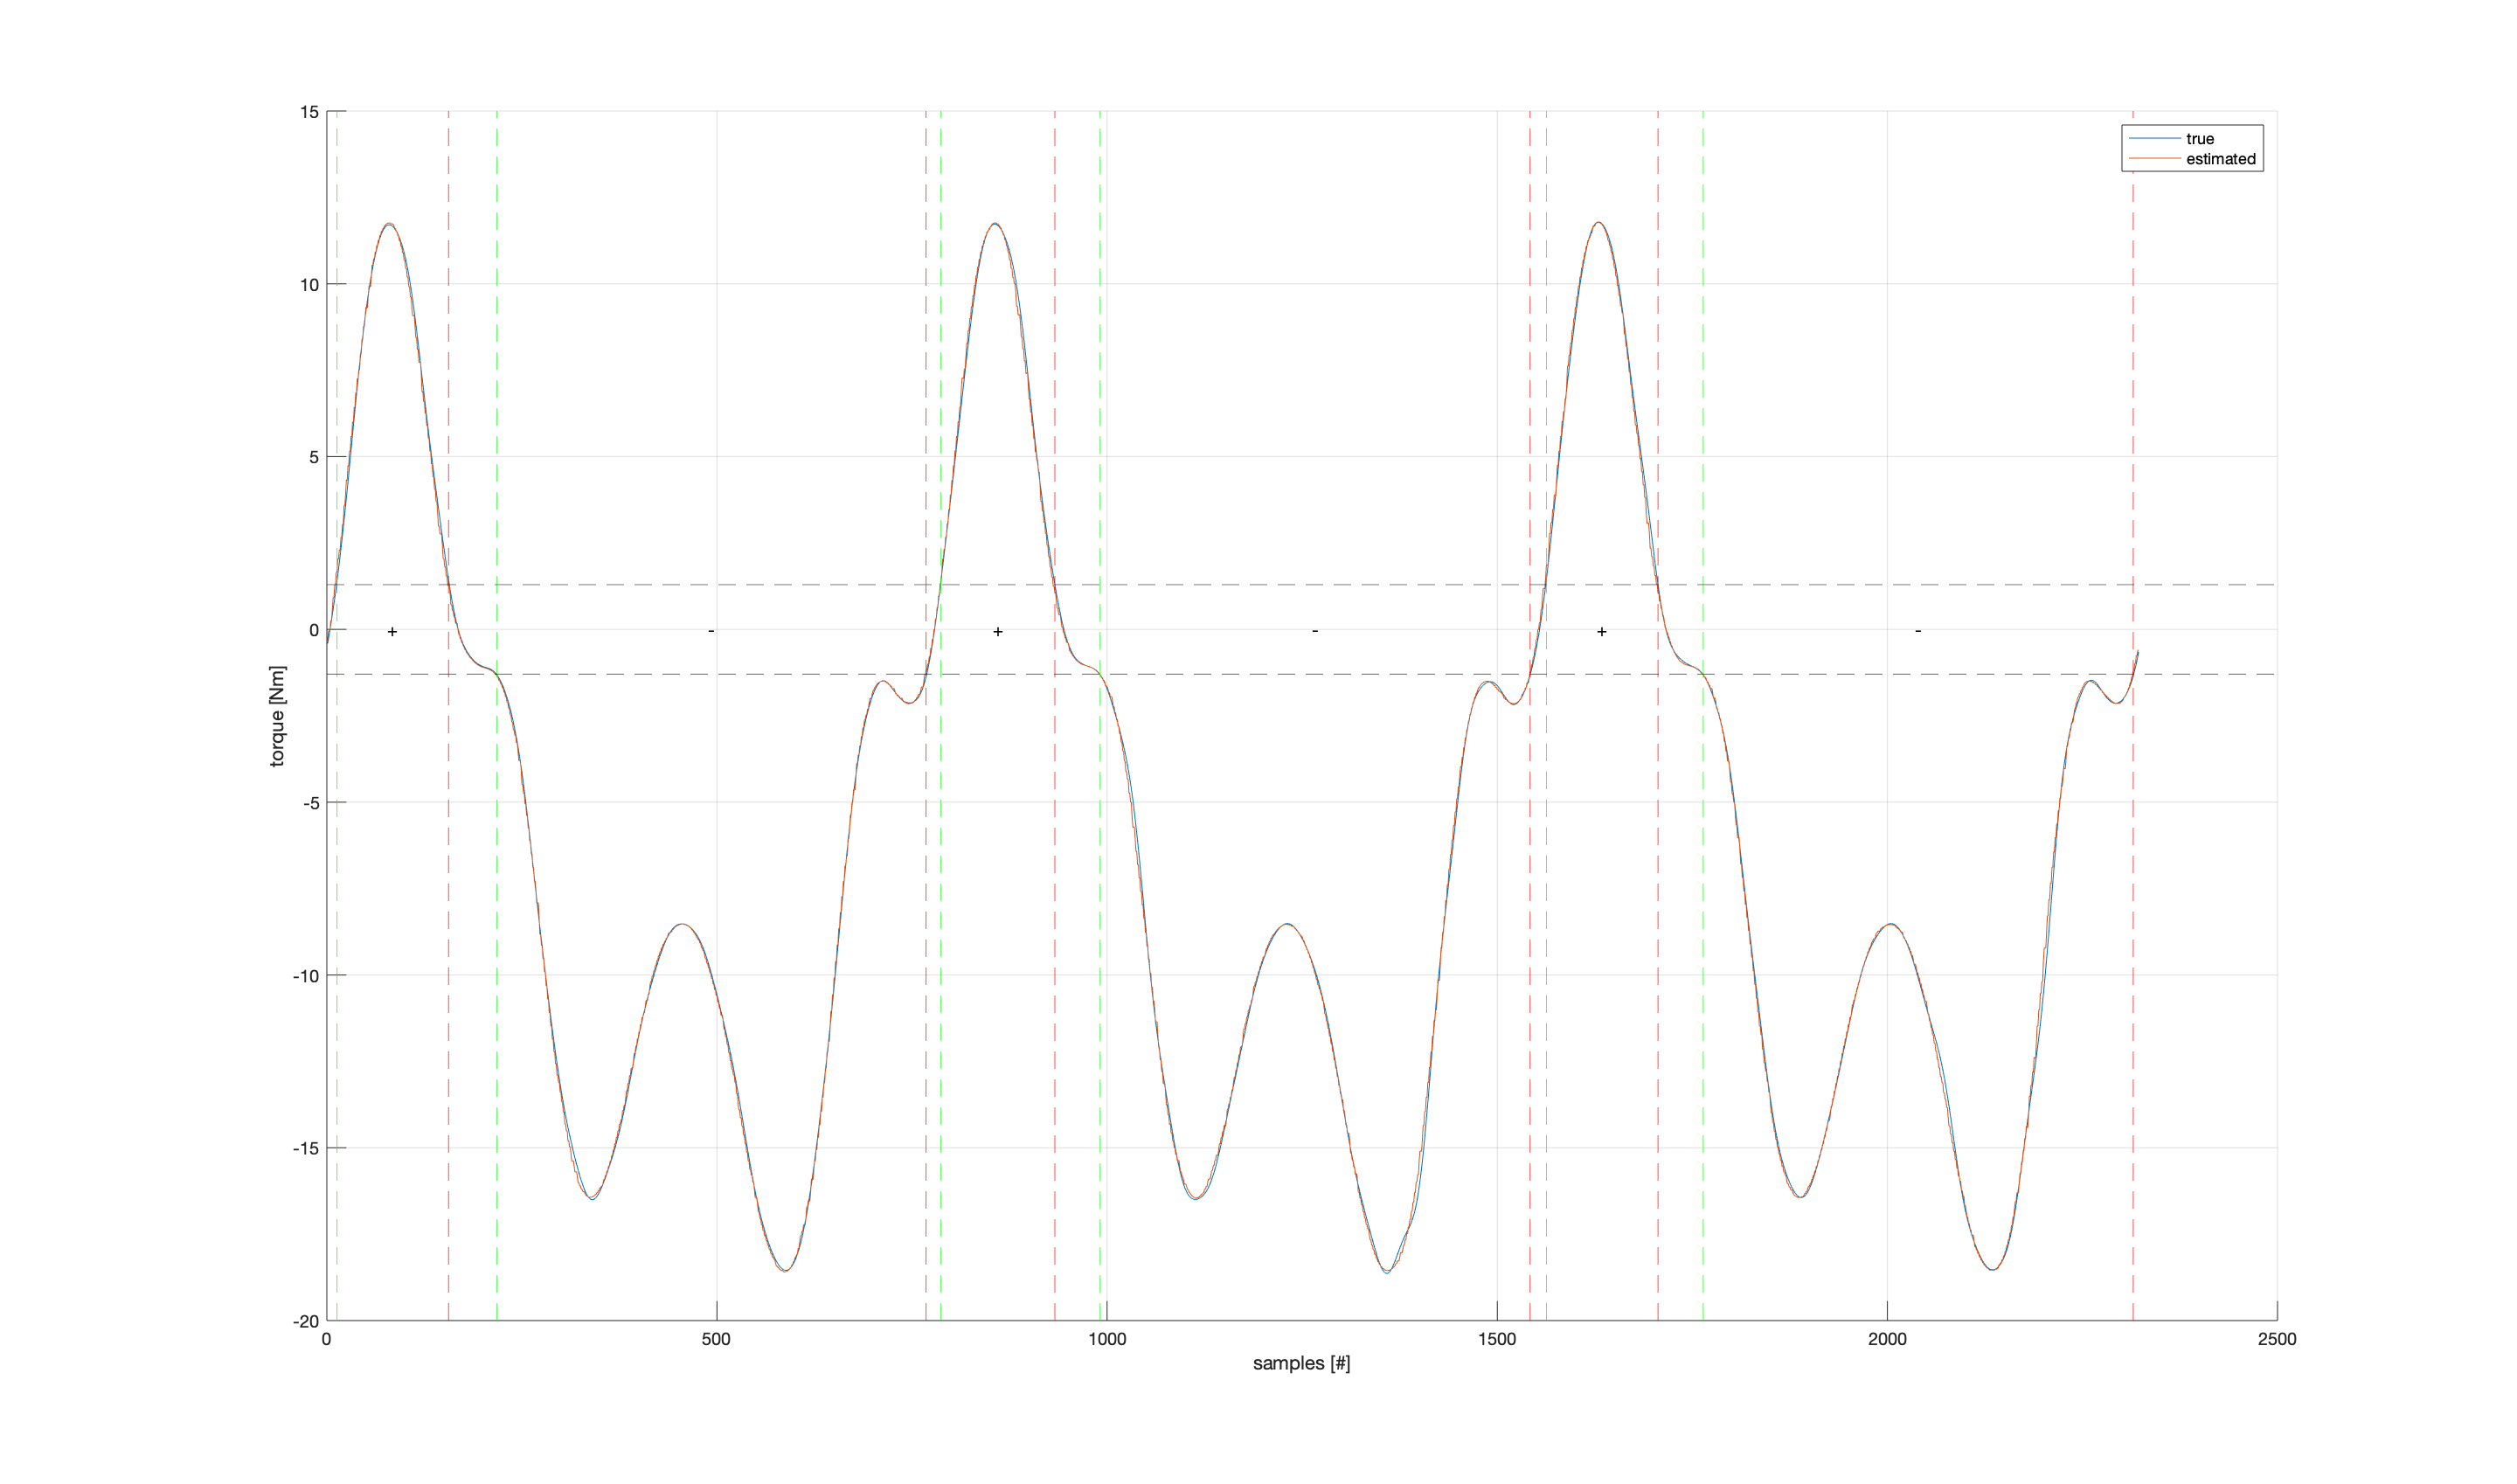
\includegraphics[width=0.8\textwidth]{images/1-dof/results_new_experiment3.png}
\caption{Plot of the reconstructed torque vs nominal torque. The gray dashed lines represent the threshold; the green dashed lines represent the start of the segment, while the red dashed lines represent the end of the segment. Samples under threshold are discarded. The signs estimated by the algorithm are reported for each segment.}
\end{figure}
\FloatBarrier
\paragraph{Experiment 4} The estimated dynamic coefficients without torque signs are:

\[\begin{bmatrix}
\pi_1  \\ \pi_2 
\end{bmatrix}=\begin{bmatrix}
24.4473 \\ 0.9756
\end{bmatrix}\]

The norm of the error is 0.6996.
\begin{figure}[!htbp]
\centering
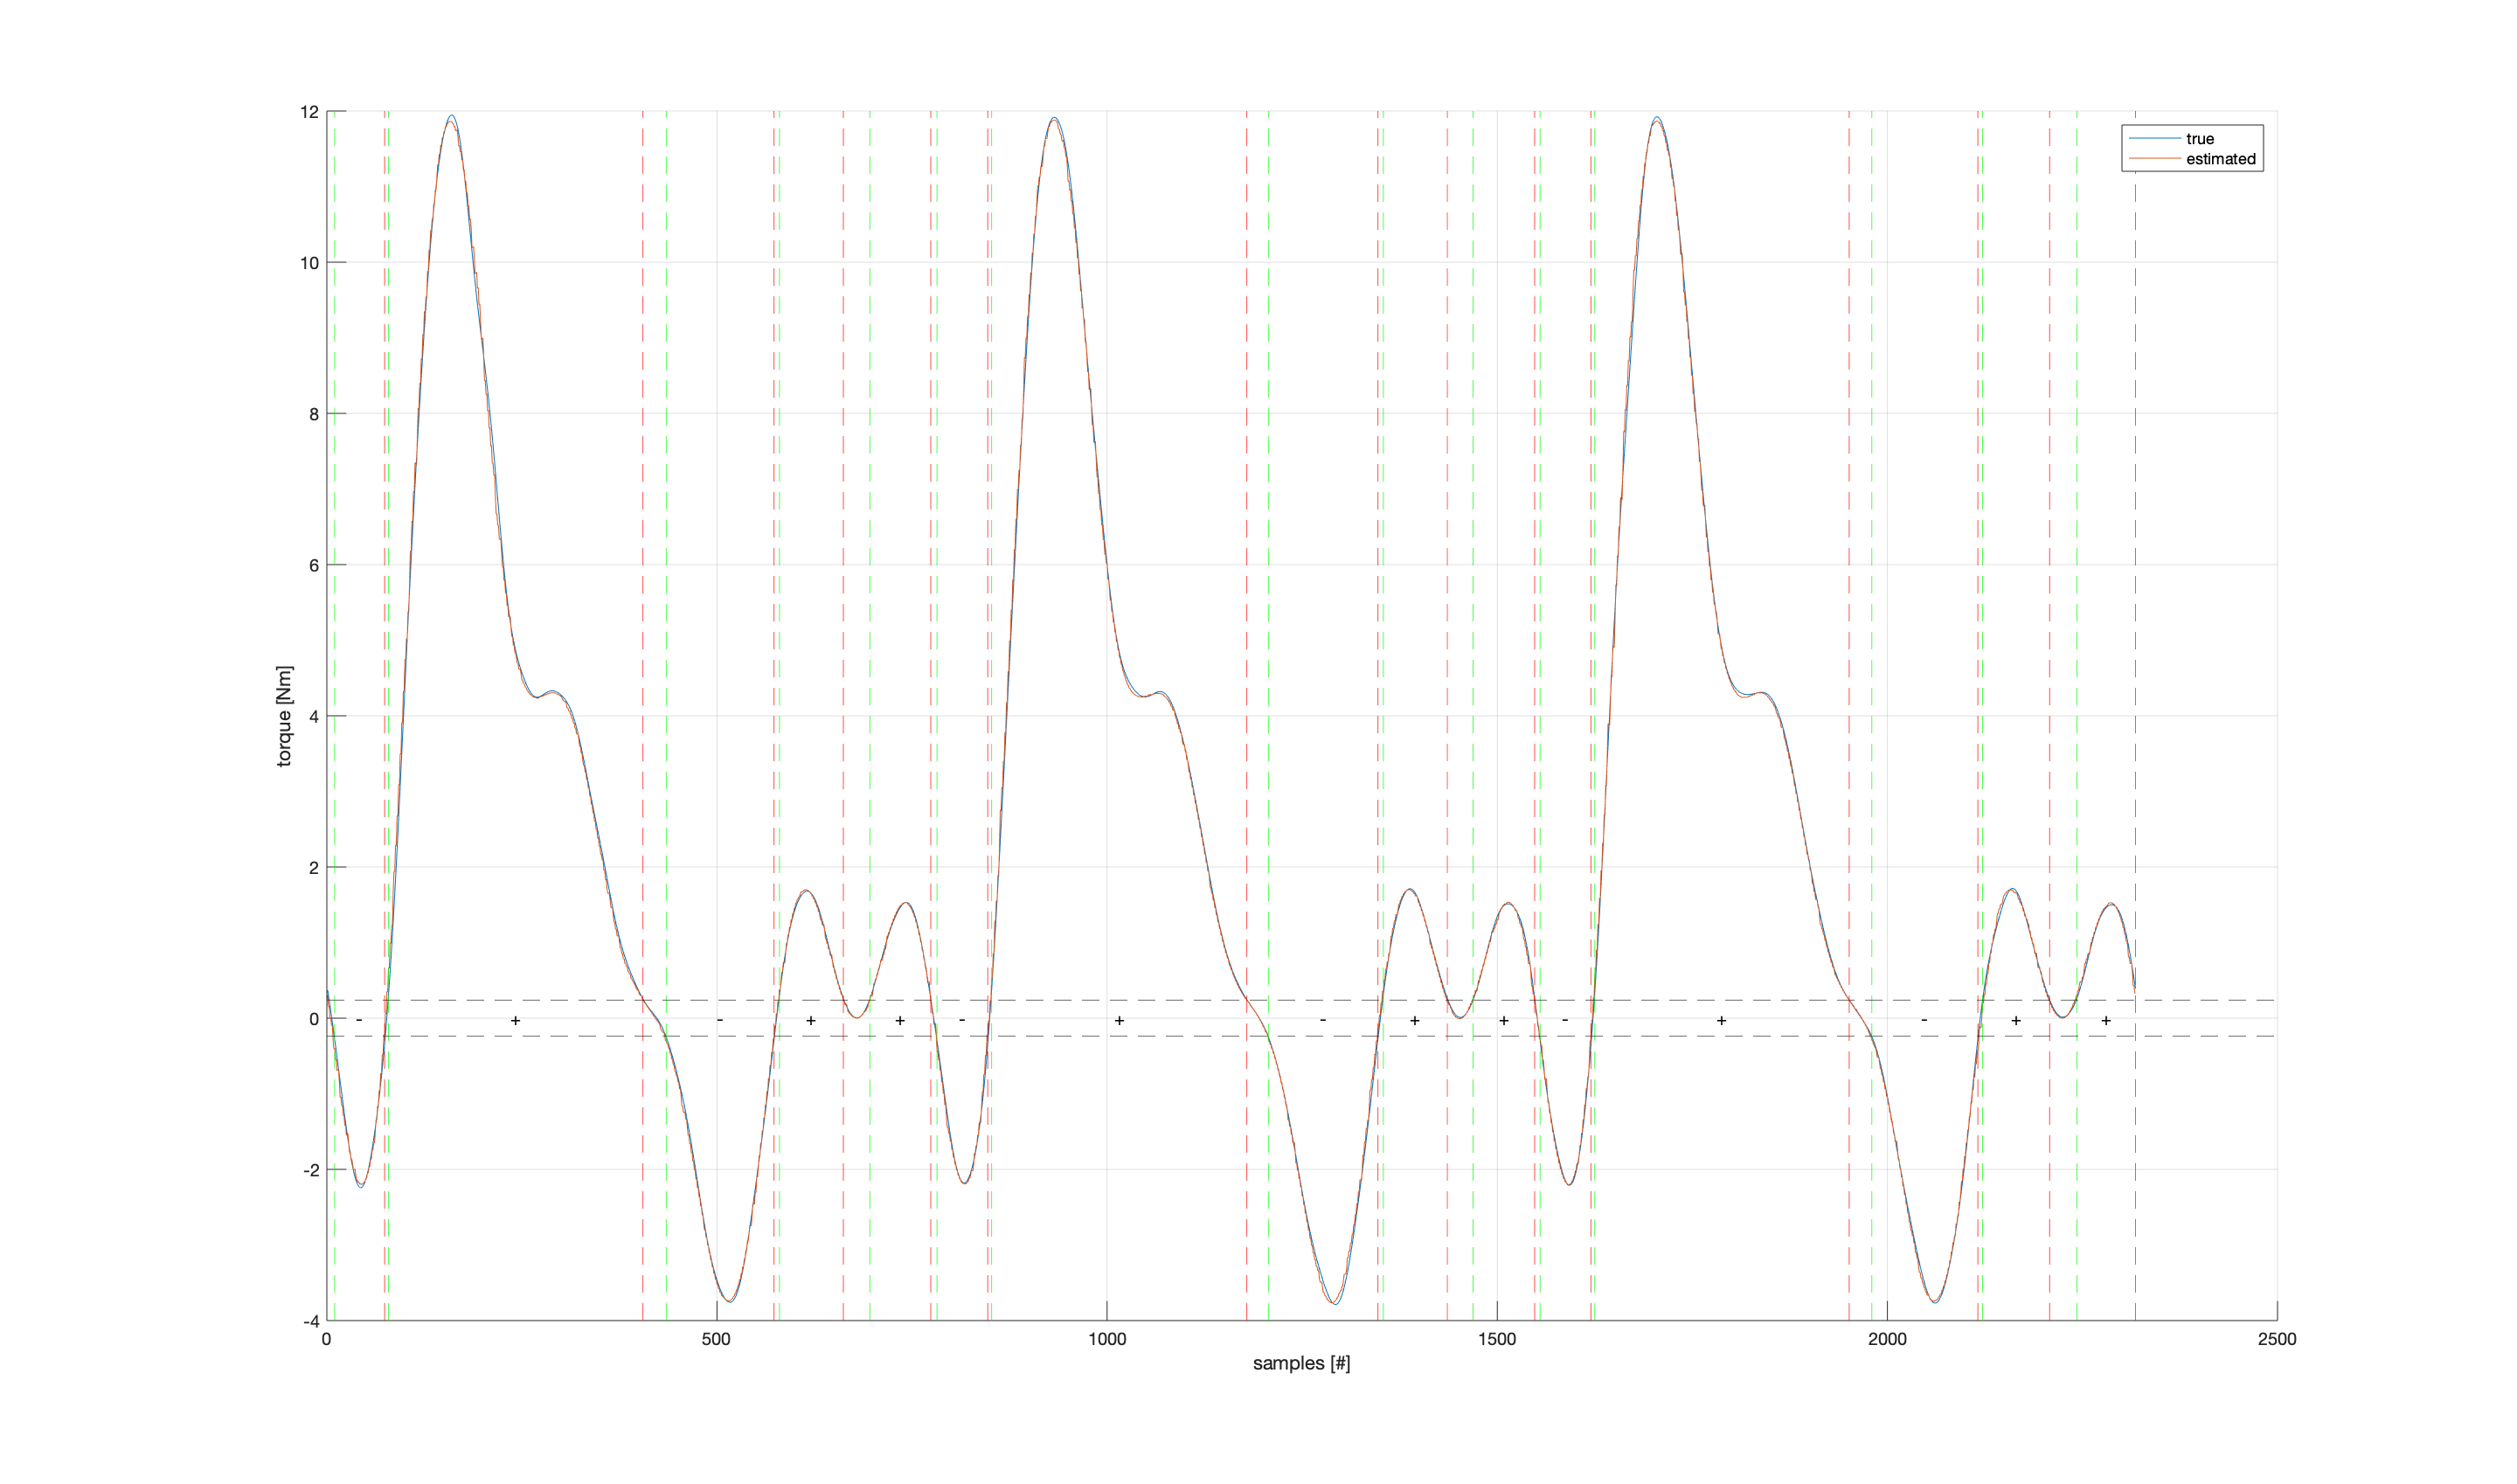
\includegraphics[width=0.8\textwidth]{images/1-dof/results_new_experiment4.png}
\caption{Plot of the reconstructed torque vs nominal torque. The gray dashed lines represent the threshold; the green dashed lines represent the start of the segment, while the red dashed lines represent the end of the segment. Samples under threshold are discarded. The signs estimated by the algorithm are reported for each segment.}
\end{figure}
\FloatBarrier
\section{3R spatial robot}
aaa
\subsection{Denavit-Hartenberg}
\paragraph{}
\FloatBarrier
\begin{table}[!htbp]
\centering
\begin{tabular}{|c|cccc|}
\hline
& $\alpha$ & a & d & $\theta$\\
\hline
link 1 & $\pi$/2 & 0 & $L_1=0.3$ & $q_1$\\
link 2 & 0 & $L_2=0.3$ & $-d_2=-0.09$ & $q_2$\\
link 3 & 0 & $L_3=0.2$ & 0 & $q_3$\\
\hline
\end{tabular}
\end{table}
\paragraph{Frame 1}
\begin{center}
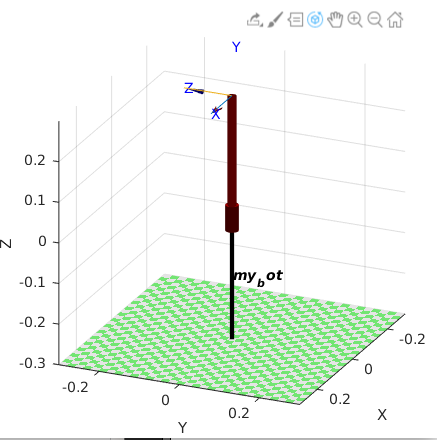
\includegraphics[width=0.5\textwidth]{images/frame1.png}
\end{center}
\paragraph{Frame 2}
\begin{center}
\begin{figure}[!htb]
   \begin{minipage}{0.33\textwidth}
     \centering
     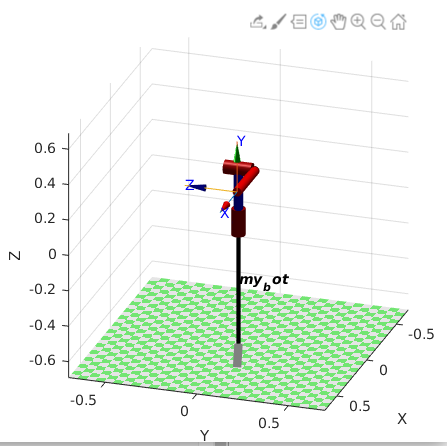
\includegraphics[width=\linewidth]{images/frame2.png}
   \end{minipage}\hfill
   \begin{minipage}{0.33\textwidth}
     \centering
     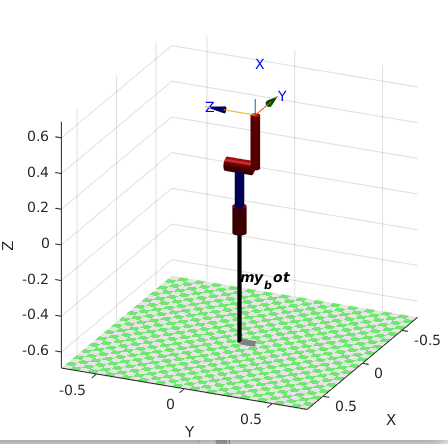
\includegraphics[width=\linewidth]{images/frame2_q2_90.png}
   \end{minipage}\hfill
   \begin{minipage}{0.33\textwidth}
     \centering
     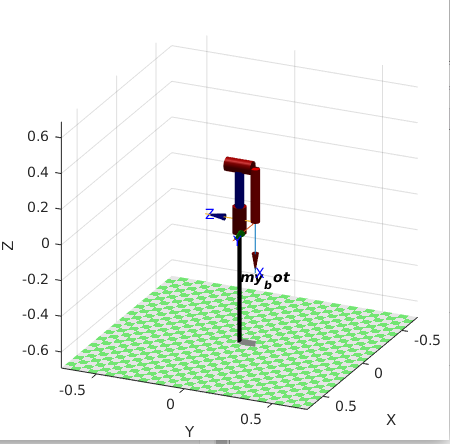
\includegraphics[width=\linewidth]{images/frame2_q2_-90.png}
   \end{minipage}
   \caption{(a) $q_2$ = 0; (b) $q_2$ = 90 deg; (c) $q_2$ = -90 deg}
\end{figure} 
\end{center}
\paragraph{Frame 3}
\begin{center}
\begin{figure}[!htb]
   \begin{minipage}{0.33\textwidth}
     \centering
     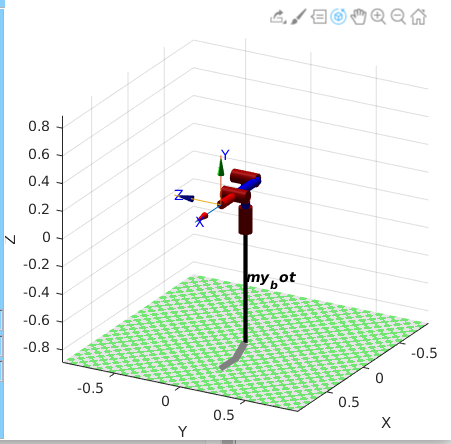
\includegraphics[width=\linewidth]{images/frame3.png}
   \end{minipage}\hfill
   \begin{minipage}{0.33\textwidth}
     \centering
     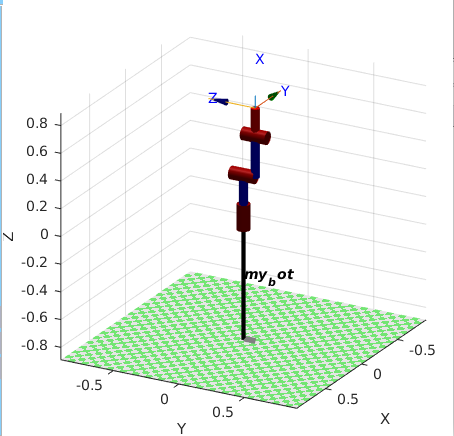
\includegraphics[width=\linewidth]{images/frame3_q2_90.png}
   \end{minipage}\hfill
   \begin{minipage}{0.33\textwidth}
     \centering
     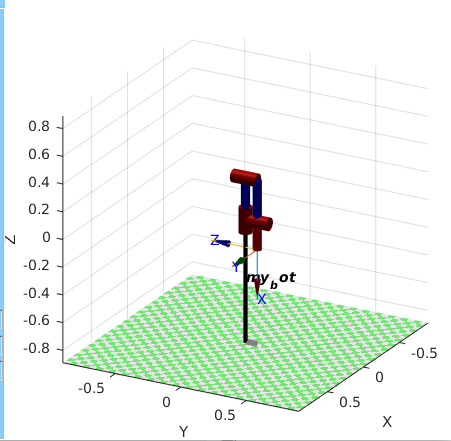
\includegraphics[width=\linewidth]{images/frame3_q2_-90.png}
   \end{minipage}
   \caption{(a) $q_2$ = 0, $q_3$ = 0; (b) $q_2$ = 90 deg, $q_3$ = 0; (c) $q_2$ = -90 deg, $q_3$ = 0}

\end{figure} 
\end{center}
\begin{center}
\begin{figure}[!htb]
   \begin{minipage}{0.33\textwidth}
     \centering
     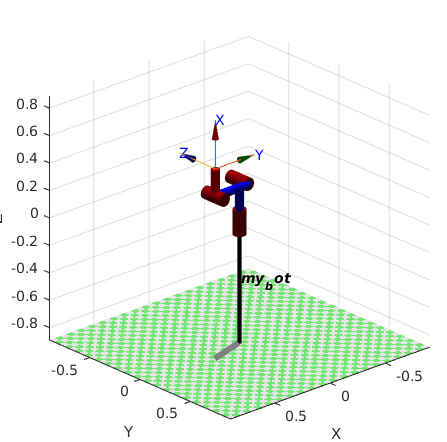
\includegraphics[width=\linewidth]{images/frame3_q2_0_q3_90.png}
   \end{minipage}\hfill
   \begin{minipage}{0.33\textwidth}
     \centering
     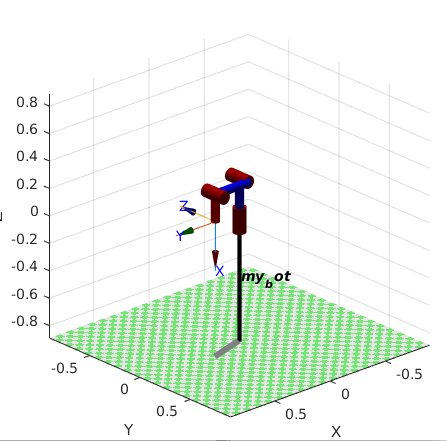
\includegraphics[width=\linewidth]{images/frame3_q2_0_q3_-90.png}
   \end{minipage}\hfill
   \begin{minipage}{0.33\textwidth}
     \centering
     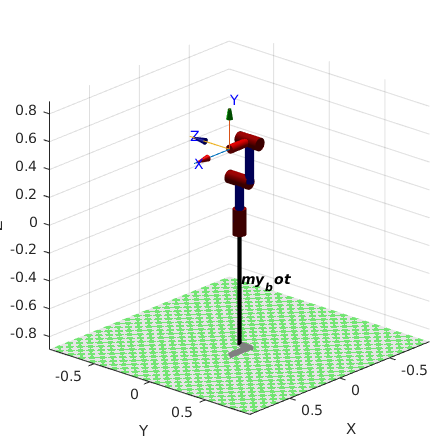
\includegraphics[width=\linewidth]{images/frame3_q2_90_q3_-90.png}
   \end{minipage}
   \caption{(a) $q_2$ = 0, $q_3$ = 90 deg; (b) $q_2$ = 0 deg, $q_3$ = -90 deg; (c) $q_2$ = 90 deg, $q_3$ = -90 deg}

\end{figure} 
\end{center}
\FloatBarrier

\subsection{Centers of Mass}
\[r_{c1}=\begin{pmatrix}
0\\
-0.15\\
0\\
\end{pmatrix} = \begin{pmatrix}
0\\
-a\\
0\\
\end{pmatrix}
\]
\[r_{c2}=\begin{pmatrix}
-0.15\\
0\\
-0.06\\
\end{pmatrix} = \begin{pmatrix}
-b\\
0\\
-c\\
\end{pmatrix}
\]
\[r_{c3}=\begin{pmatrix}
-0.10\\
0\\
0\\
\end{pmatrix}=\begin{pmatrix}
-d\\
0\\
0\\
\end{pmatrix}
\]
\[a=0.15;\qquad b=0.15;\qquad c=0.06;\qquad d=0.10 
\]
\end{document}
